\documentclass[review]{elsarticle}
\usepackage{lipsum}
\usepackage[inline]{enumitem}
\usepackage{enumerate}
\usepackage{multirow}
\makeatletter
\def\ps@pprintTitle{%
 \let\@oddhead\@empty
 \let\@evenhead\@empty
 \def\@oddfoot{}%
 \let\@evenfoot\@oddfoot}
\makeatother
\usepackage{lineno,hyperref}
\modulolinenumbers[5]

\journal{Journal of \LaTeX\ Templates}

%%%%%%%%%%%%%%%%%%%%%%%
%% Elsevier bibliography styles
%%%%%%%%%%%%%%%%%%%%%%%
%% To change the style, put a % in front of the second line of the current style and
%% remove the % from the second line of the style you would like to use.
%%%%%%%%%%%%%%%%%%%%%%%

%% Numbered
%\bibliographystyle{model1-num-names}

%% Numbered without titles
%\bibliographystyle{model1a-num-names}

%% Harvard
%\bibliographystyle{model2-names.bst}\biboptions{authoryear}

%% Vancouver numbered
%\usepackage{numcompress}\bibliographystyle{model3-num-names}

%% Vancouver name/year
%\usepackage{numcompress}\bibliographystyle{model4-names}\biboptions{authoryear}

%% APA style
%\bibliographystyle{model5-names}\biboptions{authoryear}

%% AMA style
%\usepackage{numcompress}\bibliographystyle{model6-num-names}

%% `Elsevier LaTeX' style
\bibliographystyle{elsarticle-num-names}
%\usepackage{pgfplots}
%\usepackage{natbib}
%\bibliographystyle{plainnat}
%%%%%%%%%%%%%%%%%%%%%%%

\begin{document}

\begin{frontmatter}

\title{Evaluating the Performance of Clone Detection Tools in Detecting Cloned Co-change Candidates}
%\tnotetext[mytitlenote]{Put some text for title note}

% %% Group authors per affiliation:
% \author{Md Nadim, Manishankar Mondal, Chanchal K. Roy}
% \ead{\{mdn769, mshankar.mondal, chanchal.roy\}@usask.ca}
% \address{Department of Computer Science, University of Saskatchewan, Saskatoon, Canada}

\begin{abstract}
Most changes in software systems are done by reusing existing code pieces, which creates source code clones in the codebase. These code clones may need to be changed together (co-changed) to maintain consistency in a software system during software evolution. Detecting cloned co-change candidates is essential for clone-tracking. Earlier studies showed that clone detection tools could be used to enhance the performance of finding cloned co-change candidates. Though there are several studies to evaluate the clone detection tools based on their accuracy in detecting cloned fragments, we found no study which compares different clone detection tools from the perspective of detecting cloned co-change candidates. In this study, we explore this dimension of code clone research. We used 12 different configurations of nine promising clone detection tools to identify cloned co-change candidates from eight open-source C and Java-based subject systems of various sizes and application domains and compared the performance of those clone detection tools in detecting cloned co-change fragments. Evaluated rank list and relevant analysis of obtained results provide valuable insights and guidelines about selecting the clone detection tools, which can enrich a new dimension of code clone research in change impact analysis of software systems.  
\end{abstract}

\begin{keyword}
Clone Detection; Cloned Co-change Candidates; Commit operation; Software Maintenance and Evolution
\end{keyword}

\end{frontmatter}

\linenumbers

\section{Introduction}
\label{introduction-cochage}
The comparative performance of different clone detection tools in detecting cloned co-change candidates never been investigated even though there is an availability of may clone detection tools. Detecting cloned co-change candidates is one of the vital software maintenance activities, and an earlier study \cite{Mondal:Association:Rules} showed the use of a clone detector (i.e., Nicad) could enhance the performance of such activities. Therefore, it is essential to compare the promising clone detectors in this perspective to find out the most promising tools which can be used in detecting cloned co-change candidates. Besides, it is also essential to investigate whether a clone detection tool performs well in detecting clone fragments from the codebase and is useful in detecting cloned co-change candidates?  The absence of such a study mainly motivates us to do this investigation. Clone detectors combine similar code fragments that meet certain similarity thresholds (i.e., 70\%) into clone groups. The clone group may contain two or more similar code fragments known as clone pairs (if all the groups contain exactly two similar code fragments) or clone class (it may contain two or more similar code fragments). As the fragments in such a group are identical, they should also show similar functionalities in the software system, which implies that if we want to change any of the code fragments in a clone group, other fragments in that group should also have similar change (co-changed) to keep the consistent behavior of the software system. This assumption leads us to the possibility that all the clone class members should be clone co-change candidates of each other, and whenever any of those fragments are modified, the developer should do a similar modification in all the other fragments of that class. We utilize those clone classes and pairs extracted from the subject systems using different clone detection tools to predict cloned co-change candidates.

Finding the co-change candidates of a target code fragment is also known as change impact analysis \cite{book-change-impact} in the literature.  \citet{Mondal:Association:Rules} investigated whether a clone detection tool can enhance the performance of an evolutionary coupling based tool in finding change impact set or co-change candidates. They performed their investigation using Nicad for detecting both the regular and micro-clones and found that the use of detected clone results significantly enhances the performance of Tarmaq \cite{TarmaqChangeImpact}. As they only analyzed Nicad's use, in this study, we wanted to compare some other promising clone detection tools to find whether these tools can perform better for detecting co-change candidates. Besides, \citet{CLEVER-JIT} also used the Nicad clone detection tool to recommend qualitative fixes to developers on how to fix risky (may create inconsistencies in the system) commits on 12 Ubisoft systems. They first identified risky commits using Random Forest Classifier \cite{RandomForestAlgo} based detection model and then use the Nicad clone detection tool to find out its similar commit(s) whose fix is already available in the history of the software system. Then they recommended the best-selected fixes to software developer for fixing the identified risky commit. Their study showed that at least one Ubisoft software developer accepts 66.7\% of their recommended fixes. Although their study is on a specific commercial software system and its developers, we believe clone detectors should also contribute to finding similar buggy commits and their fixes in other commercial and open-source software ecosystems. These studies motivate us to do this study where we compared 12 clone detection techniques, and the findings of our study suggest important guidelines to select clone detectors for doing change impact analysis. This study's outcomes will help for the successful integration of best performing clone detection tools with change impact analysis tools to identify risky commit and its possible fixes during commit operations.   

Software developers do the changes in a software system through some commit operations in its version control system, which could be related to each other or independent \cite{Mondal:Co-change-recommendation, Mondal:Connectivity:co-changed}. A set of change requests may come for different purposes, such as maintaining the evolving requirements and discovery of new bugs (problems/ issues), and developers mainly follow those requests and perform commit operations during software evolution. Thus, a single commit operation may contain both related and independent changes.  The related changes are known as the co-change candidates in literature \cite{Mondal-2014-PRC-2597073-2597104rankingCoChange}. Some of them may contain enough similarity in source code from clone class or pair, and some others may have differences in the source code. The code fragments that have differences in the source code may still experience a change simultaneously (co-changed) because of their functional dependency or coupling with each other.  A change done in a code fragment might need to be reflected in all of its co-change fragments to ensure consistent evolution of software systems \cite{Mondal:Association:Rules, Mondal:Context:Adaptation:Bugs}. Missing any of the co-change fragments to do proper change along with its target fragment may induce bug or inconsistency in the software system \cite{Judith:Bug:Replication, Judith:Micro:Regular:Clone}. 

We have evaluated four different configurations of CloneWorks \cite{CloneWorks-Jeff} and eight other clone detectors in our investigation. Therefore, we have 12 separate implementations of clone detection tools (we will consider them as 12 separate tools in the rest of this paper).  We apply these tools on thousands of commit operations from the evolutionary histories of eight open-source software systems having different sizes in source code and application domains. Configuration of the clone detection tools are given in Table \ref{tab:tool-configurations} and the software systems used in this study are reported in Table \ref{tab:subject-systems-cc}.

Based on this study, we answered the following research questions:

\vspace{0.15cm}
\noindent
\textbf{RQ1: }How can we compare different clone detection tools based on the performance in detecting cloned co-change candidates? 
 
\vspace{0.15cm}
\noindent
\textbf{RQ2: }What are the deciding factors for the performance variance of different clone detectors in detecting cloned co-change candidates?

\vspace{0.15cm}
\noindent
\textbf{RQ3: }Do the source code processing techniques (Pattern/Token/Text-based processing) of the clone detection tools have any impact on their performance in detecting co-change candidates?

\vspace{0.15cm}
\noindent
\textbf{RQ4: }Do clone detection tools designed for detecting different types of clones (Type 1, 2, 3) work differently in detecting cloned co-change candidates?

To the best of our knowledge, study to compare clone detection tools considering a particular maintenance perspective (such as their performance in detecting cloned co-change candidates during software evolution) has never been done earlier. One can assume that a clone detector, which is good in detecting cloned fragments, might also be good in detecting cloned co-change candidates. We wanted to verify this assumption in this exploratory study practically. We selected 12 implementations of clone detectors detecting different types of clone fragments to evaluate their performance in detecting cloned co-change candidates. Our investigation and analysis find that the clone detectors that detect Type-3 clones and perform pattern-based source code processing are significantly good in detecting cloned co-change candidates. Our investigation also shows that tools which provide more number of clone fragments and cover more source code lines are also good in detecting cloned co-change candidates. We have created a final rank list of the clone detection tools based on our investigation, which is shown in Table \ref{tab:final-ranking-sum-of-ranks}, where we have considered the ranking of the clone detectors in each of the subject systems to make a final ranking. A clone detector performed well in most of the subject systems got a higher rank in this ranking table. Considering the rank list in Table \ref{tab:final-ranking-sum-of-ranks} we find:
\begin{enumerate*}[label=(\roman*)]
  \item the tools which are good in detecting all types (1/2/3) of clones are also good in detecting cloned co-change candidates. 
  \item Top two of the tools in the final rank list are the Type-3 configurations of CloneWorks (one splits source files with lines and the other split the source file with tokens to process it before detecting clone fragments), and other following clone detectors which perform well are Deckard and CCFinder. Therefore, to detect cloned co-change candidates, those tools (all are pattern and token-based) are the best choices compared to the other tools used in this study.
  \item From this ranking, we can also find that text-based clone detectors (such as Duplo or CloneWorks Type-1) are not suitable for detecting co-change candidates.
  \item Our comparison in Figure \ref{fig:AverageLineCoveredPerSS} also shows that the clone detectors which detect a higher number of clone fragments and cover a higher number of unique lines in the source files are performing good in detecting cloned co-change candidates. 
\end{enumerate*}
We have also done the Wilcoxon Signed-Rank Test \cite{wilcoxon-signed-rank-test, wilcoxon-signed-rank-test-rosner} to verify whether the F1~Scores in all the eight subject systems of the tools which got higher ranks in the final rank list (Table \ref{tab:final-ranking-sum-of-ranks}) are significantly better compared to the other clone detection tools or not. The results of our significance test are described in Section \ref{sec-wilcoxon-singed-rank-test}. A summary of our significance test results is in Table \ref{tab:cochange-wilcoxon-rank-test}, which shows that four out of the 12 clone detection techniques of this study perform significantly better than the other techniques in detecting cloned co-change candidates.
%\vspace{0.5mm}

We organized this paper in the following sections: Some related works are described in Section \ref{the-related-works}, our methodology is in Section \ref{the-methodology}, we described the experimental result in Section \ref{the-experimental-result}, the discussion is in section \ref{the-discussion}, Section \ref{the-threat-validity} explains some possible threats to validity, and we conclude our paper in Section \ref{the-conclusion-cochange}.

This paper is a significant extension of our previous work \cite{nadim-iwsc-2020} on detecting cloned co-change candidates using different clone detectors. Our previous work answered two research questions by analyzing six clone detectors on six open-source software systems. Our earlier study's two research questions showed that even though a tool that is good in detecting clone fragments from software systems may not be useful in detecting cloned co-change candidates. The tools that detect a large number of clone fragments and cover more unique lines in the source files are found suitable in predicting cloned co-change candidates. We extend our previous work by answering two additional research questions (RQ3, RQ4) to find more specific reasons for the variation of the performance by clone detectors in detecting co-change candidates. We have also increased the previous study's generalizability by adding two more software systems as subject systems and three more clone detection tools with four different configurations of CloneWorks (Type-1, Type-2 blind, Type-3 pattern, and Type-3 token), totaling eight subject systems and 12 clone detector executions. Therefore, our implementation has been upgraded from 6X6 to 12X8 (Clone detector X Subject Systems) in the study's current version. In this study, we have shown that the performance of clone detection tools in detecting cloned co-change fragments depends on some specific factors of clone detectors such as (i) the number of discovered clone fragments, (ii) the number of unique lines covered by those clone fragments, (iii) source file processing techniques, and (iv) type of detected clones. 

\vspace{2mm}
\section{Related Work}
\label{the-related-works}
Several studies \cite{Roy09comparisonand, jeff-evaluating, 4288192Comparison, ScenarioBasedComparison} have focused on ranking different clones detection tools based on their performance and accuracy in detecting different types of clone fragments. \citet{BaileyBurdComparison}  has compared three clones and two plagiarism detecting tools based on their performance in detecting cloned code in a single file or across different files. \citet{4288192Comparison} made a framework for comparing the performance of different clone detection tools from eight large C and Java programs having the size of source code almost 850 KLOC. One of the authors of this study also manually validated the dataset used in this study.  \citet{EvaluateRefactoring} compared three representative clone detection techniques from a refactoring perspective. Their criteria for comparison were the portability, kinds of clone reported, scalability, number of false positive, and number of useless clone detection from the results of those clone detection techniques. \citet{jeff-evaluating} reported ConQAT, iClones, NiCad, and SimCAD as excellent tools for detecting clones of all the three types (Type-1, Type-2, Type-3) based on their evaluation of eleven modern clone detection tools using four benchmark frameworks. \citet{Roy09comparisonand} did a qualitative comparison and evaluation of the latest clone detection approaches and tools, and made a benchmark called BigCloneBench \cite{BigCloneBenchCKRoyJRCordy} BigCloneBench included eight million manually verified clone pairs in a large inter-project source code dataset where the number of projects is larger than 25,000 and lines of code are above 365 million. They classify, compare, and evaluate different clone detectors based on the following point of view, (i) how the set of attributes in the different code fragments are overlapped, and (ii) what are the scenarios of creating Type-1, Type-2, Type-3, and Type-4 clones.  They also explained the procedure of using the result of their study for selecting the appropriate clone detectors in the context of particular application areas and restrictions. 

Besides proposing new clone detection mechanisms, some studies also compared their tools with a few existing tools. \citet{astDetectionComparisonBellon} utilizes suffix trees in abstract syntax trees to detect code clones and compared their technique with other few techniques using the Bellon benchmark for clone detectors \cite{DucasseStringMatchingCloneBallon}. Two other studies \cite{DucasseStringMatchingCloneBallon, CloneIntermediateRepresentationBallon} also measured the performance of their proposed clone detectors (based on string comparison and intermediate source transformation) utilizing Bellon’s framework. 

\citet{CloneIntermediateRepresentationBallon} showed their tool provides improved recall (with a slight drop in precision) compared to the source based clone detectors, and it also detects Type-3 clones. They also utilized Bellon’s corpus in their study and compared their technique with other standalone string and token-based clone detectors where they found little higher precision. All the studies that compared different clone detectors focused on the precision, recall, computational complexity, and memory used or detecting a specific type of clone fragments such as Type-1, Type-2, Type-3, or Type-4 during the detection approach of duplicated code in a codebase. 

Our study to compare clone detectors is entirely different from the previous comparisons. We do not want to compare clone detection tools based on the capability to detect clones. Our point of interest is to detect co-change candidates during the software commit operations. \citet{Mondal-2014-PRC-2597073-2597104rankingCoChange} used the detected clone results of Nicad to predict and rank the co-change candidates by analyzing evolutionary coupling from previously done change history. However, no other clone detection tool is included in their study to compare the performance of different clone detection tools in the prediction and rank of those co-change candidates. We extended our previous study \cite{nadim-iwsc-2020} to compare the performance of 12 implementations of nine different clone detection tools based on the performance of detecting clone co-change candidates using eight software systems written in C and Java programming languages.  We found no other study which has performed a similar comparison of clone detectors. We believe this investigation is the first to compare clone detection tools' in the perspective of specific software maintenance acclivity (doing change impact analysis by detecting cloned co-change candidates). 

%\vspace{1mm}
\section{Methodology}
\label{the-methodology}
To complete this study, we divide this study in several steps and performed following set of operations. 

\subsection{Selecting the subject systems:} 
The popularity of programming language and the availability of substantial revisions are both considered essential factors for selecting subject systems for this study. TIOBE Programming Community index \cite{TIOBE2019} (an indicator of the popularity of programming languages) recorded Java as the highest and C as the second-highest popular programming language based on the data of more than ten years. This index motivates us to take subject systems written in C and Java programming language. To produce a generalizable result, the availability of a substantial amount of revisions and diversity in size and application domain is also an essential factor for subject systems. Considering all of these factors, we have selected the subject systems. Table \ref{tab:subject-systems-cc} includes the list of our eight subject systems of divers sizes and application domains, four of which are written in C programming language, and the other four are in Java. 

%%% Beginning of Subject Systems Table
\begin{table}[htbp] 
\caption{\label{tab:subject-systems-cc}\textsc{Subject Systems}}
\centering
\begin{tabular}{|c|c|l|c|}
\hline
\textbf{Systems} & \textbf{Language} & \multicolumn{1}{c|}{\textbf{Domains}} & \textbf{Revisions} \\ \hline \hline
Brlcad           & C              & Computer Aided Design                 & 2115               \\ \hline
Camellia         & C              & Batch Job Server                      & 301                \\ \hline
Carol            & Java           & Game                                  & 1700               \\ \hline
Ctags            & C              & Code Def. Generator                   & 774                \\ \hline
Freecol          & Java           & Game                                  & 1950               \\ \hline
Jabref           & Java           & Reference Manager                     & 1545               \\ \hline
jEdit            & Java           & Text Editor                           & 4000               \\ \hline
Qmailadmin (QMA)       & C              & Mail System Manager                   & 317                \\ \hline
\end{tabular}
\end{table}
%%%--- End of Subject Systems Table

\subsection{Identifying all the Co-change Candidates}
We prepared the cloned co-change candidates by processing all the revisions of all the subject systems which we mention in Table \ref{tab:subject-systems-cc}. To identify the cloned co-change candidates, we first extracted all the changes in each of the revisions using the Unix diff command. All the changes that happened in a single revision are co-change of each other. Considering each of the changes as target change, we tried to predict all the other code fragments changed in the same revision (i.e., co-changed) utilizing each of the clone detection tools. We find some change fragments whose co-change candidates are not detected by any of the 12 clone detection tools used in this study, which are considered as independent change fragments and excluded while calculating the performance of clone detection tools to be compared with each other. Considering only dependent (cloned) changes while calculating the performance measures (precision, recall, and F1~Scores) is necessary to make a fair comparison among the clone detection tools. Finally, we compare all the tools based on their F1~Scores in detecting those cloned co-change candidates.

\subsection{Preparing Cloned Co-change Candidates (Ground Truth)} 
Even though we have extracted all the changes between two adjacent revisions (i.e., revision n and n+1), we can not fully guarantee that all the changes are actually co-change candidates of each other. Some changes might not depend on any other changes, and they may change independently. The inclusion of such dissimilar changes into our calculation can drop the detection accuracy of clone detectors. We considered excluding those co-changes that are not detected by any 12 clone detection techniques to minimize the effect of them on the calculated performance measures (precision, recall, F1~Score). As none of the clone detectors in this study finds any co-change candidates, we considered those changes as dissimilar or independent changes. 


We have used eight open-source software systems, having varieties of size and application domains as subject systems in this study. The list of subject systems are in Table \ref{tab:subject-systems-cc}. To detect cloned co-change candidates from those subject systems, we executed 12 clone detection tools (Table \ref{tab:tool-configurations}) and analyzed obtained results to evaluate the performance of those clone detection tools. Our analysis evaluates these clone detection tools' performance in successfully suggesting actual co-change candidates (ACC) during the software evolution and determines the ranking of these tools based on this performance evaluation. To start our primary analysis, we need to take some considerations to resolve the following issues. 

%%% Start of Summary Data
\begin{table}[htbp]
\centering
\caption{\label{tab:data-summary}\textsc{Summary of Data Processed}}
\small\addtolength{\tabcolsep}{-4.2pt}
\begin{tabular}{|l|c|c|c|c|c|c|c|c|}
\hline
\textbf{\begin{tabular}[c]{@{}l@{}}Revisions/ SS\end{tabular}} & \textbf{Brlcad} & \textbf{Camellia} & \textbf{Carol} & \textbf{Ctags} & \textbf{Freecol} & \textbf{Jabref} & \textbf{jEdit} & \textbf{QMA} \\ \hline \hline
Processed                                                                     & 2113            & 301               & 1700           & 774            & 1001             & 1540            & 215            & 317                                                            \\ \hline
\begin{tabular}[c]{@{}l@{}}Experiencing \\ change\end{tabular}                                                         & 660             & 163               & 454            & 447            & 836              & 860             & 145            & 35                                                             \\ \hline
\begin{tabular}[c]{@{}l@{}}Experiencing more \\ than one change\end{tabular}  & 553             & 155               & 430            & 330            & 833              & 755             & 145            & 25                                                             \\ \hline
\end{tabular}
\end{table}
%%%-------------------------------

\subsection{Selecting the clone detectors:} Considering some related studies about the ability of clone detection tools in detecting clone fragments, we have selected some promising mechanisms for this study, which can identify all the Type-1, Type-2, and Type-3 clones. We have taken CloneWorks \cite{CloneWorks-Jeff} as it is considered a fast and flexible clone detector for large-scale near-miss clone detection experiments. CloneWorks tool provides the ability to change its processing mechanism by changing its configuration files. We applied four different configurations of CloneWorks to detect Type-3 Pattern, Type-3 Token, Type-2 Blind, and Type-1 clones for investigating the impact of the types of clones in detecting co-change candidates. We included Duplo \cite{DuploCloneDetection} as another type-1 clone detector for comparing with type-1 clones of CloneWorks in this investigation.  ConQAT \cite{conqat-clone-detecion}, iClones \cite{4812755iclones}, NiCad \cite{5970189Nicad}, and SimCAD \cite{6613857Simcad} have been reported as very good tools for detecting all types of clones in the study of \citet{jeff-evaluating}. Besides these, CCFinder \cite{CCFinderCloneDetection}, Deckard \cite{4222572Deckard}, iClones and NiCad are often considered as common examples of modern clone detectors that support Type-3 clone detection. CCFinder is known as a multi-linguistic token-based code clone detection system for large scale source code. The inclusion of CCFinder enriched the variation of detected clone fragments in the extended study.  To make more comparison of the performance of type-1 clones in detecting co-change candidates, we added Duplo in our study. We included Simian \cite{simianlink} in our analysis because of its ability to find cloned codes by line-by-line textual comparison supporting identifier renaming with a fast detection speed on the large repository and widespread use in several related studies \cite{simian-used-1, Wang-2013-SBC-2491411-2491420, impact-clone-maintenance, Cheung-clones-javascript, cloning-gnome-project}. NiCad, SimCAD, and Simian extract cloned code fragments from a software system's codebase using textual similarity among different code pieces. Deckard makes vector representation of different code fragments and then utilizes tree representation of those vectors to calculate the similarity among code pieces.  CCFinder, ConQAT, and iClones extract tokens from the source code and then use those tokens to find similar fragments.

\subsection{Selecting Identical Parameter Configurations of the Clone Detectors} 
Taking an identical configuration of different clone detectors while applying them on different subject systems to identify cloned code fragments is essential. We compared them with each other based on their capability to successfully suggest co-change candidates, and identified clones from each clone detectors have a crucial impact on their performance in suggesting cloned co-change candidates. \citet{Wang-2013-SBC-2491411-2491420} reported taking different configurations of clone detectors may change the result of detected clones, and the result can be very good or terrible depending on the taken configuration. This scenario is known as a confounding configuration choice problem, and it should be handled very carefully while determining the configuration to be taken to detect cloned fragments using any clone detection tool. 
Our configuration of different tools is shown in Table \ref{tab:tool-configurations}. As our goal is to compare different tools with each other, configuring them similarly while clone detection will provide consistent results for a fair comparison. We have also tried to have identical configuration values to \citet{jeff-evaluating}, which they conducted to compare different clone detectors based on their efficiency in detecting cloned fragments. We provided a 70\% similarity threshold for all the clone detection tools (except Deckard), which takes similarity dissimilarity value as a parameter. We have used 85\% as the similarity threshold for Deckard because, in an initial manual inspection of the detected results, we found a massive number of clone fragments in Deckard's results compared to the other clone detectors while using the similarity threshold 70\% like the others. We also identified many clone classes having the same fragments (self duplicate fragments) as the clone fragments of that class. To minimize those duplicated fragments, we tried other similarity threshold values such as 75\%, 80\%, and  85\%. We found that increasing the similarity threshold reduces the self duplicated fragments, and we took the detected clone results applying the 85\% similarity threshold for Deckard in all the subject systems. \citet{jeff-evaluating} also used 85\% similarity while running Deckard for Mutation Framework. We have also selected identical parameter values such as the minimum number of tokens, the minimum number of lines for different clone detection tools. As we wanted to compare different clone detectors based on their capability of successfully suggesting co-change candidates, it was essential to configure them identically during detecting clones from our subject systems.

\subsection{The overall approach} 

Figure \ref{fig:CalculatingCC} provides a demonstration of our overall process in calculating each of the clone detection tools' performance metric values. Let us consider that 21 changes, C1 to C21, occurred in the codebase during a particular commit operation in a subject system. We extract these changes utilizing the UNIX diff command. If we consider any changes (i.e., C1) as the target change, the other 20 changes (i.e., C2 to C21) will be considered the actual co-change candidates of C1.  


We apply different clone detection tools to detect these co-change candidates considering C1 as the target change. Let us assume, Deckard can detect five (i.e., C2, C6, C8, C15, C21) from those 20 fragments as co-change candidates of C1. Similarly, NiCad can detect four (i.e., C5, C10, C16, C18) of them as co-change candidates of C1. We continued the same approach for all the clone detection tools to detect co-change candidates of C1. Obtained results from all the tools provide ten unique change fragments (C2, C5, C8, C15, C21, C5, C8, C10, C15, C21) by taking a union of the individual detected results of all the clone detectors. We will then consider those ten unique change fragments as cloned co-change candidates and calculate each of the clone detectors' precision and recall based on their number of detection among those cloned co-change candidates. 

We finally calculated average recall, average precision in each of the subject systems for all the clone detection tools. We compare the clone detection tools based on the F1~Scores calculated by using the average recall and precision shown in the equation \ref{eq-f1-score}. Figure \ref{fig:AveragePrecisionRecall} shows the bar chart of Average Recall and Average Precision drawn from our experimental results, and in Table \ref{tab:detection-f1-score}, we have given the calculated weighted average of F1~Score. According to our findings and ranking of the clone detectors (Table \ref{tab:final-ranking-sum-of-ranks}), we can conclude that CloneWorks (both two configurations, Type-3 Pattern and Token), Deckard, and CCFinder outperforms all the other tools. CloneWorks Type-2 Blind, ConQAT, and iClones fall in the following order. From the final rank list, we also see that the clone detection tools which detecting only Type-1 clones (such as Duplo, CloneWorks Type-1) are performing worst in finding co-change candidates.  We also calculated the percent of distinct lines covered in the source files (Figure \ref{fig:AverageLineCoveredPerSS}) of subject systems by the detected clone results, which shows that the clone detector which has the highest percentage of detected distinct lines as a cloned line in the codebase also performs well in detecting cloned co-change candidates.

%The number of fragments detected by a clone detector also shows  

%%% Calculating Cloned Co-change
%%%--- Bar Chart of Precision
\vspace{4mm}
\begin{figure}
\centering
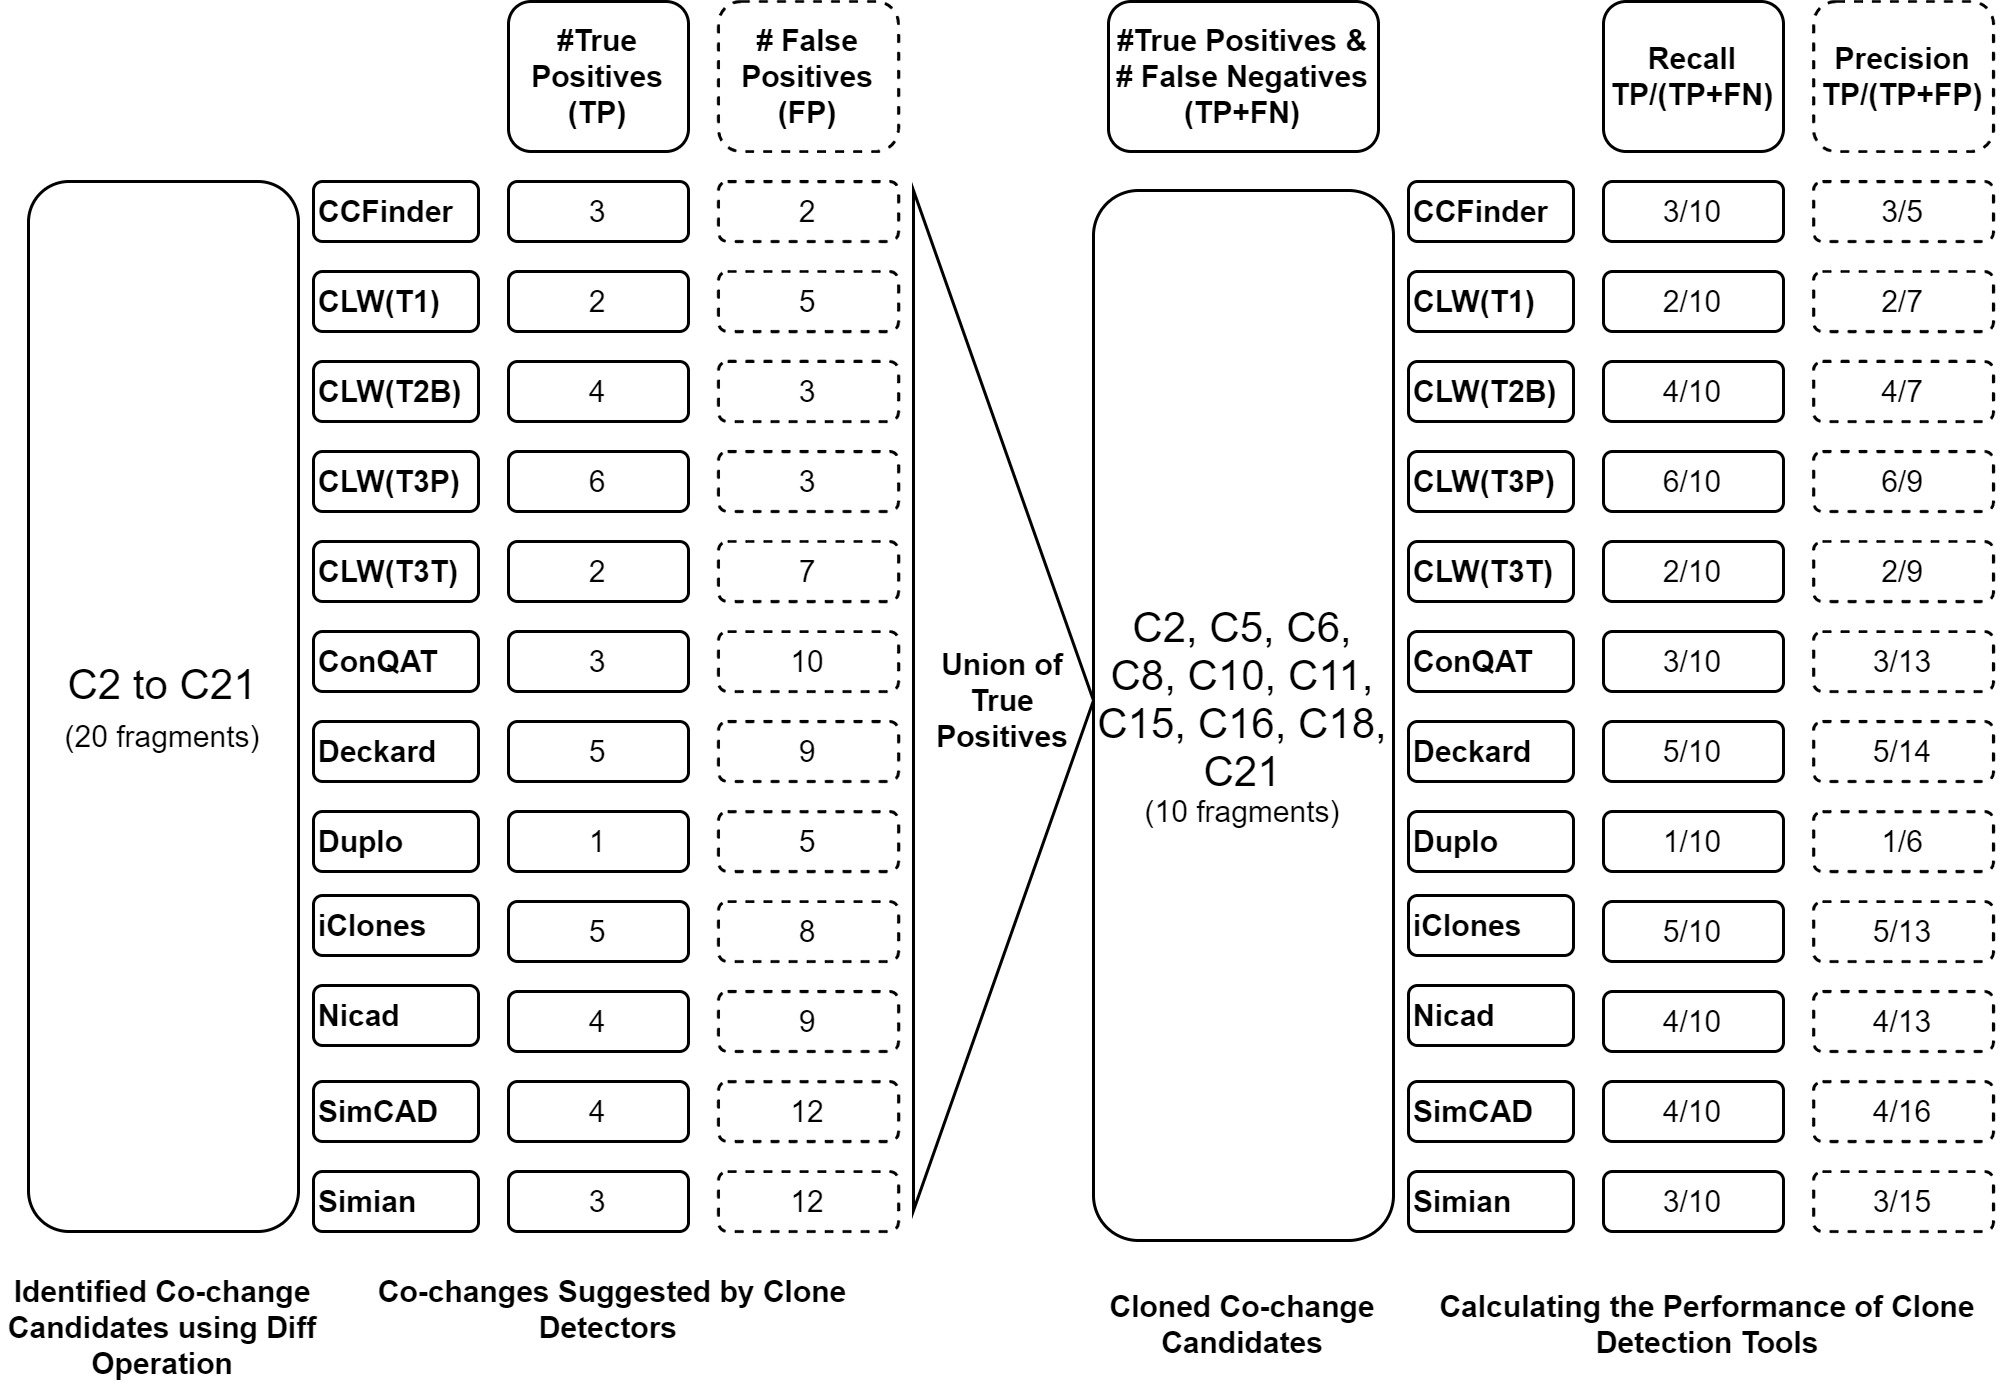
\includegraphics[width=\columnwidth] {CalculatingCC.jpg}
% Calculation of Change Intersection: SELECT COUNT(`change_id`) FROM `pre_recall_conqat` WHERE `change_detect`>0
\caption{This diagram explains how we calculated the Recall and Precision in one revision. We first identified the co-change candidates as ground truth using the Unix diff operation, then we have used the results of each of the clone detection tools to identify those co-change candidates. True Positives (TP) are the co-changes that we successfully identified using the clone detectors. Our process also provided some False Positives (FP) in each revision. To separate the cloned co-change candidates from all the previously identified co-change candidates, we took the union of all the TPs from all the clone detection tools. The Recall is the ratio of TPs and the number of cloned co-change candidates (TP+FN), and the Precision is the ratio of TPs and the number of total co-change suggestions (TP+FP). We repeated the process for all the revisions of all the subject systems used in our investigation.}
\label{fig:CalculatingCC}
\end{figure}
%%% ==================

Our overall processing is performed in some distinct steps.  Initially, we downloaded all the source files of all the subject systems' revisions from their respective SVN repositories. We then applied \textbf{diff} operation between each file of a revision with the corresponding file in the next revision to extract follwoing change information such as (i) name of the file which is changed, (ii) the beginning line number of the respective change, and (iii) the ending line number of the change. We did the change extraction for each revision (excluding the last one) of all the subject systems. After detecting all the changes, we started the clone detection on all the subject systems' revisions using all the clone detection tools. We started our principal analysis to find each of the clone detection tools' accuracy after having the result of all the clone detectors and change information from all the revisions. 

Figure \ref{fig:CalculatingCC} demonstrates the overall procedure of calculating the accuracy of different clone detectors used in this study. Let us assume, while examining a specific commit operation, we found the number of fragments changed with this commit is $n$. In each step, we consider one of those fragments as the target fragment and the remaining $n-1$ fragments as the actually co-changed candidates for that target fragment. Among the $n-1$ fragments, there could be some fragments that have changed independently. We have described the procedure to exclude those independent fragments in the introduction (Section \ref{introduction-cochage}) of this study. After excluding independent fragments, we get the \textbf{Actually Cloned Co-change} (ACC) for each of the target fragments. 

Now, we find the cloned fragment from the results of clone detectors intersecting with the target fragment. The other fragments in the intersecting clone fragment class are considered the \textbf{Predicted Cloned Co-change} (PCC) candidates. We now determine how many of these PCC intersect with the ACC to obtain the number of detected cloned co-change candidates by the clone detector. 

These counts of predicted and actually co-changed candidates are considered as the \textbf{true positives} to calculate Recall, Precision, and F1~Score. We calculate these using the following equations (Eq. 1, 2, and 3). 

\begin{equation}
    Recall = \frac{|PCC \cap ACC|}{|ACC|}
\end{equation}

\begin{equation}
    Precision = \frac{|PCC \cap ACC|}{|PCC|}
\end{equation}

\begin{equation}
\label{eq-f1-score}
    F1~Score = \frac{2 \times Precision \times Recall}{Precision + Recall}
\end{equation}

\vspace{1mm}
We repeat the calculating process of Recall and Precision for all the changes in each of the subject systems with the detected clone fragments generated by all the clone detection tools. We then calculate the F1~Score of the clone detectors for each of the subject systems by taking the average values of Recall and Precision, which is reported in Table \ref{tab:detection-f1-score}. We reported the ranking of the tools considering individual ranks in each of the subject systems in Table \ref{tab:final-ranking-sum-of-ranks}.

\subsection{Producing the final rank list:} To produced the final rank list of 12 clone detection techniques, we considered their performance in all the eight individual subject systems. Our ranking approach is demonstrated in Table \ref{tab:final-ranking-sum-of-ranks}, which shows both the ranks in individual subject systems and final overall ranking for each of the clone detectors. S1, S2, ....., S8 are the subject systems used in this study, and these are in the same order as shown in Table \ref{tab:detection-f1-score}, which shows the F1~Scores of detecting cloned co-change candidates by each of the clone detection tools in the respective software systems. The highest F1~Score in Table \ref{tab:detection-f1-score} got rank-1, and similarly the lowest one got rank-12 in the respective position of Table \ref{tab:final-ranking-sum-of-ranks}. Therefore, every clone detection technique has eight rank values (smaller value represents the better performance), obtained in the eight software systems. We then took the summation of those eight individual ranks for producing the overall ranking for each of the clone detection techniques. A smaller summation value of individual ranks means that the clone detector performed well in most subject systems. Based on the summation of individual rankings, we reported the final rank of each clone detection technique in the right-most column of the Table \ref{tab:final-ranking-sum-of-ranks}. 

%%% TAble Summary of Participating Tools
\begin{table}[htbp]
\centering
\caption{\label{tab:tool-configurations}\textsc{Configuration of Participating Clone Detection Tools}}
%\small\addtolength{\tabcolsep}{-1pt}
\begin{tabular}{ll}
\hline
\multicolumn{1}{|l|}{\textbf{Tools}} & \multicolumn{1}{l|}{\textbf{Configuration   for Clone Detection}}                                                                                      \\ \hline \hline
\multicolumn{1}{|l|}{CCFinder}       & \multicolumn{1}{l|}{min. size: 50 tokens, min. token types: 12}                                                                                        \\ \hline
\multicolumn{1}{|l|}{CLW(T1)}        & \multicolumn{1}{l|}{termsplit=token, termproc=Joiner}                                                                                                  \\ \hline
\multicolumn{1}{|l|}{CLW(T2B)}   & \multicolumn{1}{l|}{\begin{tabular}[c]{@{}l@{}}cfproc=rename-blind,   cfproc=abstract literal, \\ termsplit=token, termproc=Joiner\end{tabular}}       \\ \hline
\multicolumn{1}{|l|}{CLW(T3P)} & \multicolumn{1}{l|}{\begin{tabular}[c]{@{}l@{}}cfproc=rename-blind, cfproc=abstract literal,\\ termsplit=line\end{tabular}}                            \\ \hline
\multicolumn{1}{|l|}{CLW(T3T)}   & \multicolumn{1}{l|}{\begin{tabular}[c]{@{}l@{}}termsplit=token,   termproc=FilterOperators, \\ termproc=FilterSeperators\end{tabular}}                 \\ \hline
\multicolumn{1}{|l|}{ConQAT}         & \multicolumn{1}{l|}{block clones, clone   min-length=5, gap ratio=0.3}                                                                                 \\ \hline
\multicolumn{1}{|l|}{Deckard}        & \multicolumn{1}{l|}{\begin{tabular}[c]{@{}l@{}}min. size: 30   tokens, 5 token stride, \\ min. 85\% similarity\end{tabular}}                           \\ \hline
\multicolumn{1}{|l|}{Duplo}          & \multicolumn{1}{l|}{min. size: 10 lines, min. characters/line:1}                                                                                       \\ \hline
\multicolumn{1}{|l|}{iClones}        & \multicolumn{1}{l|}{\begin{tabular}[c]{@{}l@{}}minimum block: 30, minimum   clone: 50, \\ All Transformation\end{tabular}}                             \\ \hline
\multicolumn{1}{|l|}{Nicad}          & \multicolumn{1}{l|}{\begin{tabular}[c]{@{}l@{}}block clones,   blind renaming, max. threshold=0.3,\\ minimum lines=5, maximum lines=2500\end{tabular}} \\ \hline
\multicolumn{1}{|l|}{SimCAD}         & \multicolumn{1}{l|}{block clones,   Source Transformation= generous}                                                                                   \\ \hline
\multicolumn{1}{|l|}{Simian}         & \multicolumn{1}{l|}{min. size: 5   lines, normalize literals/identifiers}                                                                              \\ \hline
\multicolumn{2}{l}{\textit{\textbf{CLW:} CloneWorks; \textbf{T1:} Type-1; \textbf{T2B:} Type-2, Blind Renaming;}}  
\\
\multicolumn{2}{l}{\textit{ \textbf{T3P:} Type-3, Pattern;  \textbf{T3T:} Type-3, Token;}}    
\end{tabular}
\end{table}
%%%--- End of Summary Table
\begin{table}[htbp]
\centering
\caption{\label{tab:summary-atc-acc}\textsc{Summary of Actual Target and Co-change Candidates}}
\begin{tabular}{lcccc}
\hline
\multicolumn{1}{|c|}{\textbf{SS}}    & \multicolumn{1}{c|}{\textbf{\# ATC}} & \multicolumn{1}{c|}{\textbf{\# ACC}}  & \multicolumn{1}{c|}{\textbf{\% ATC}} & \multicolumn{1}{c|}{\textbf{\% ACC}} \\ \hline \hline
\multicolumn{1}{|l|}{Brlcad}         & \multicolumn{1}{c|}{2909}            & \multicolumn{1}{c|}{33578}            & \multicolumn{1}{c|}{7.45}            & \multicolumn{1}{c|}{1.89}            \\ \hline
\multicolumn{1}{|l|}{Camellia}       & \multicolumn{1}{c|}{8052}            & \multicolumn{1}{c|}{346140}           & \multicolumn{1}{c|}{20.61}           & \multicolumn{1}{c|}{19.46}           \\ \hline
\multicolumn{1}{|l|}{Carol}          & \multicolumn{1}{c|}{4582}            & \multicolumn{1}{c|}{254311}           & \multicolumn{1}{c|}{11.73}           & \multicolumn{1}{c|}{14.29}           \\ \hline
\multicolumn{1}{|l|}{Ctags}          & \multicolumn{1}{c|}{718}             & \multicolumn{1}{c|}{3648}             & \multicolumn{1}{c|}{1.84}            & \multicolumn{1}{c|}{0.21}            \\ \hline
\multicolumn{1}{|l|}{Freecol}        & \multicolumn{1}{c|}{6865}            & \multicolumn{1}{c|}{265213}           & \multicolumn{1}{c|}{17.57}           & \multicolumn{1}{c|}{14.91}           \\ \hline
\multicolumn{1}{|l|}{Jabref}         & \multicolumn{1}{c|}{8313}            & \multicolumn{1}{c|}{455469}           & \multicolumn{1}{c|}{21.28}           & \multicolumn{1}{c|}{25.60}           \\ \hline
\multicolumn{1}{|l|}{jEdit}          & \multicolumn{1}{c|}{5122}            & \multicolumn{1}{c|}{323277}           & \multicolumn{1}{c|}{13.11}           & \multicolumn{1}{c|}{18.17}           \\ \hline
\multicolumn{1}{|l|}{QMA}            & \multicolumn{1}{c|}{2508}            & \multicolumn{1}{c|}{97396}            & \multicolumn{1}{c|}{6.42}            & \multicolumn{1}{c|}{5.47}            \\ \hline
\multicolumn{1}{|l|}{\textbf{Total}} & \multicolumn{1}{c|}{\textbf{39069}}  & \multicolumn{1}{c|}{\textbf{1779032}} & \multicolumn{1}{c|}{\textbf{100}} & \multicolumn{1}{c|}{\textbf{100}} \\ \hline
\multicolumn{5}{l}{\textit{\textbf{SS:} Subject Systems}}                                                                                                                                         \\
\multicolumn{5}{l}{\textit{\textbf{\# ATC:} Number of   Actual Taget Changes}}                                                                                                                   \\
\multicolumn{5}{l}{\textit{\textbf{\# ACC:} Number of   Actual Co-changes}}                                                                                                                     
\end{tabular}
\end{table}
%%%--- 

\section{Experimental Result}
\label{the-experimental-result}
This section will answer the research questions based on our overall analysis and obtained results by processing each of the eight subject systems using all the 12 clone detection tool executions. 

\subsection{Answer to the \textbf{RQ1}}
\textbf{How can we compare different clone detection tools based on the performance in detecting cloned co-change candidates?}

The key experimental results are in Figure \ref{fig:AveragePrecisionRecall}, Table \ref{tab:summary-atc-acc}, Table \ref{tab:detection-f1-score}, and Table \ref{tab:final-ranking-sum-of-ranks} where Fig. \ref{fig:AveragePrecisionRecall} shows the average Recall and average Precision of each of the clone detection tools. Table \ref{tab:summary-atc-acc} shows the summary of target changes and detected co-change candidates for those target changes in each of the subject systems.  We found the highest and lowest percentage of target change and its cloned co-change candidates from Jabref and Ctags. Table \ref{tab:detection-f1-score} shows the F1~Score of each of the clone detectors in each of the subject systems. The F1~Score is calculated using Equation (3). Our experimental results concluded in Table \ref{tab:final-ranking-sum-of-ranks}, which shows that CLW(T3P), CLW(T3T), and Deckard shows top performance (Rank 1 or 2) in most of the subject systems compared to all the other tools. The summary of the results in the Table \ref{tab:final-ranking-sum-of-ranks} shows that among the subject systems, CLW(T3P) is the best in all the subject systems except Camellia and Freecol, where Deckard is showing the best performance. CLW(T3T) shows the second-best performance in most of the subject systems. An overall observation on individual rankings of different clone detection techniques reveals that CLW(T3P), Deckard, CLW(T3T), CCFinder show better performance in most of the subject systems compared to the other clone detectors. On the other hand, Duplo, CLW(T1) shows the worst performance in most subject systems. Other tools show average performance considering individual ranking in different subject systems.  CLW(T1) and Duplo obtained the bottom position in the final rank list. 

As our analysis was based on the clone grouping into class or pair provided by the clone detection tools, we found that clone detection tools' efficiency in suggesting cloned co-change candidates is mostly dependent on its effectiveness in making clone class/ pair. The tool which groups functionally similar clone fragments into a clone class/ pair effectively can perform well in successfully suggesting cloned co-change candidate(s). Different values of different clone detectors' accuracy indicate the difference in their efficiency in this research domain. 

%%%--- Bar Chart of Recall
\begin{figure}
\centering
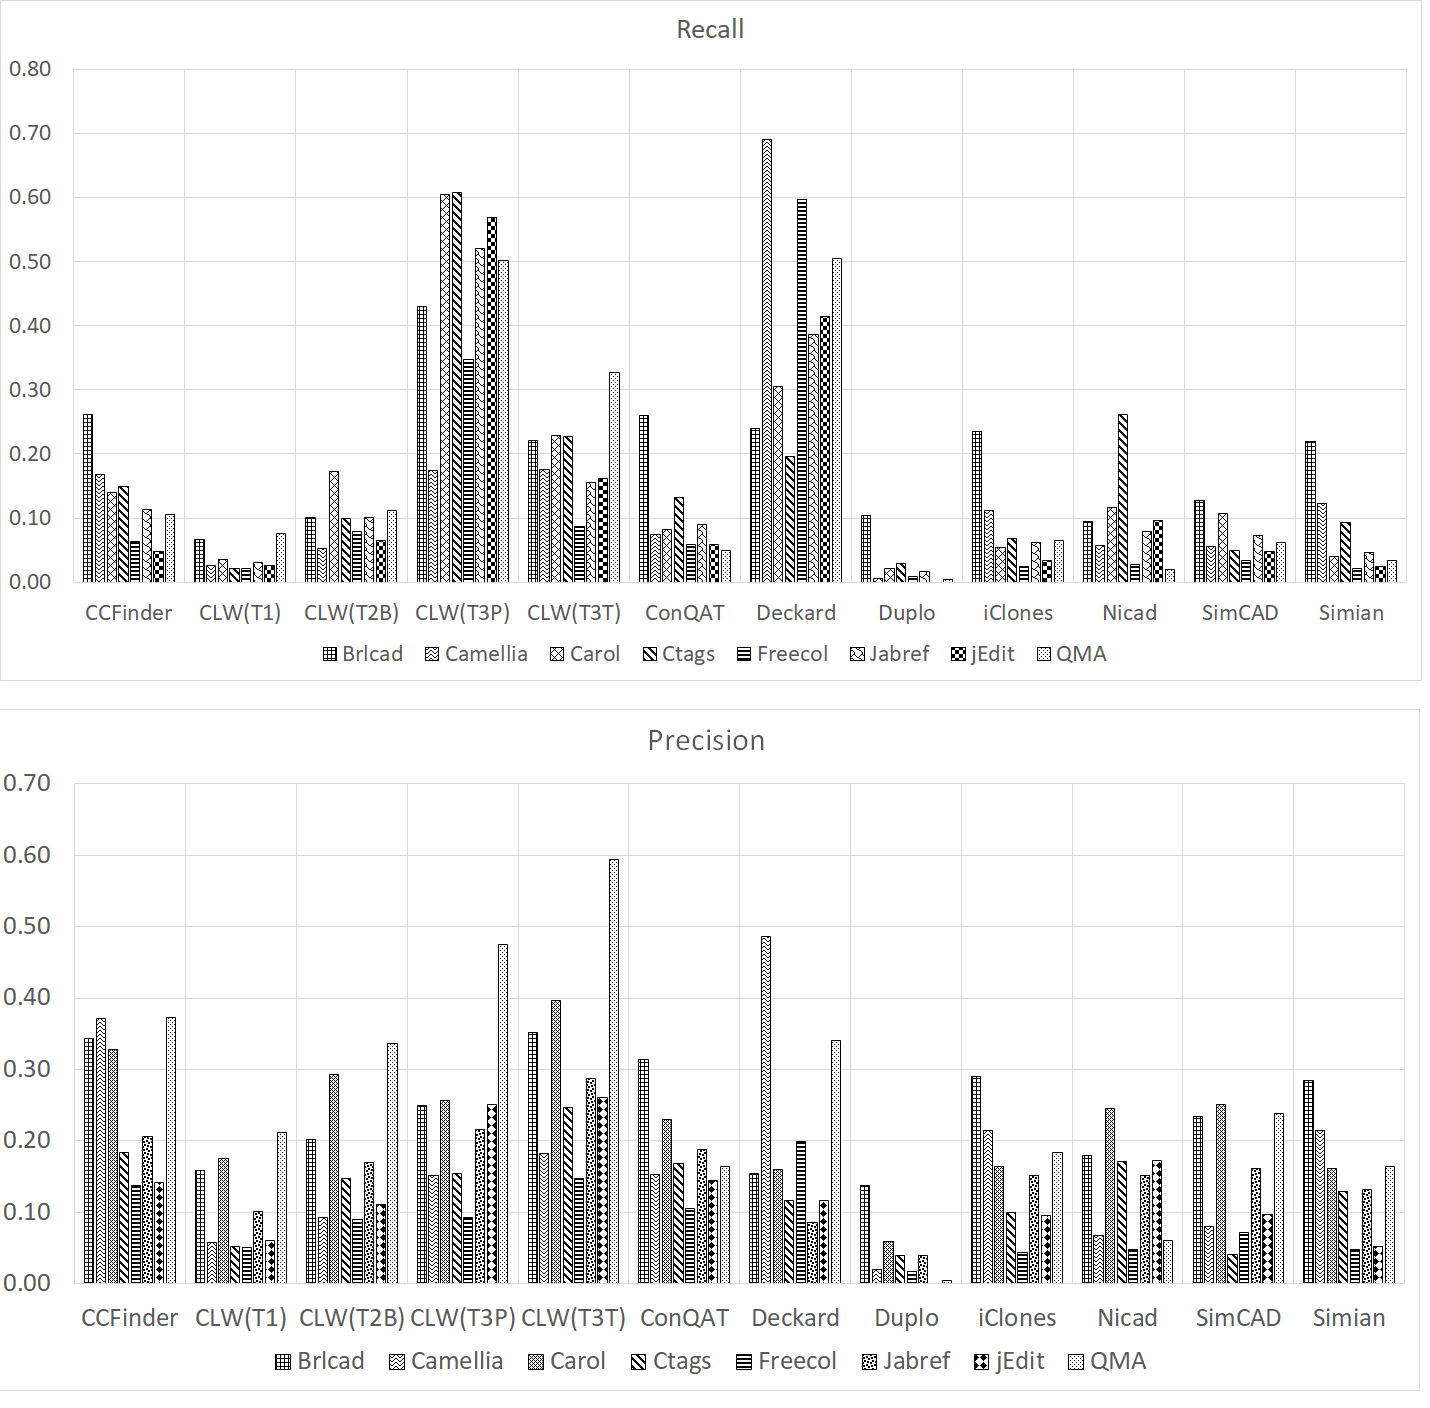
\includegraphics[width=\textwidth] {AveragePrecisionRecall.png}
\caption{Average recall and precision of different tools}
\label{fig:AveragePrecisionRecall}
\end{figure}
%%% ==================

% %%%--- Bar Chart of Precision
% \begin{figure}
% \centering
% 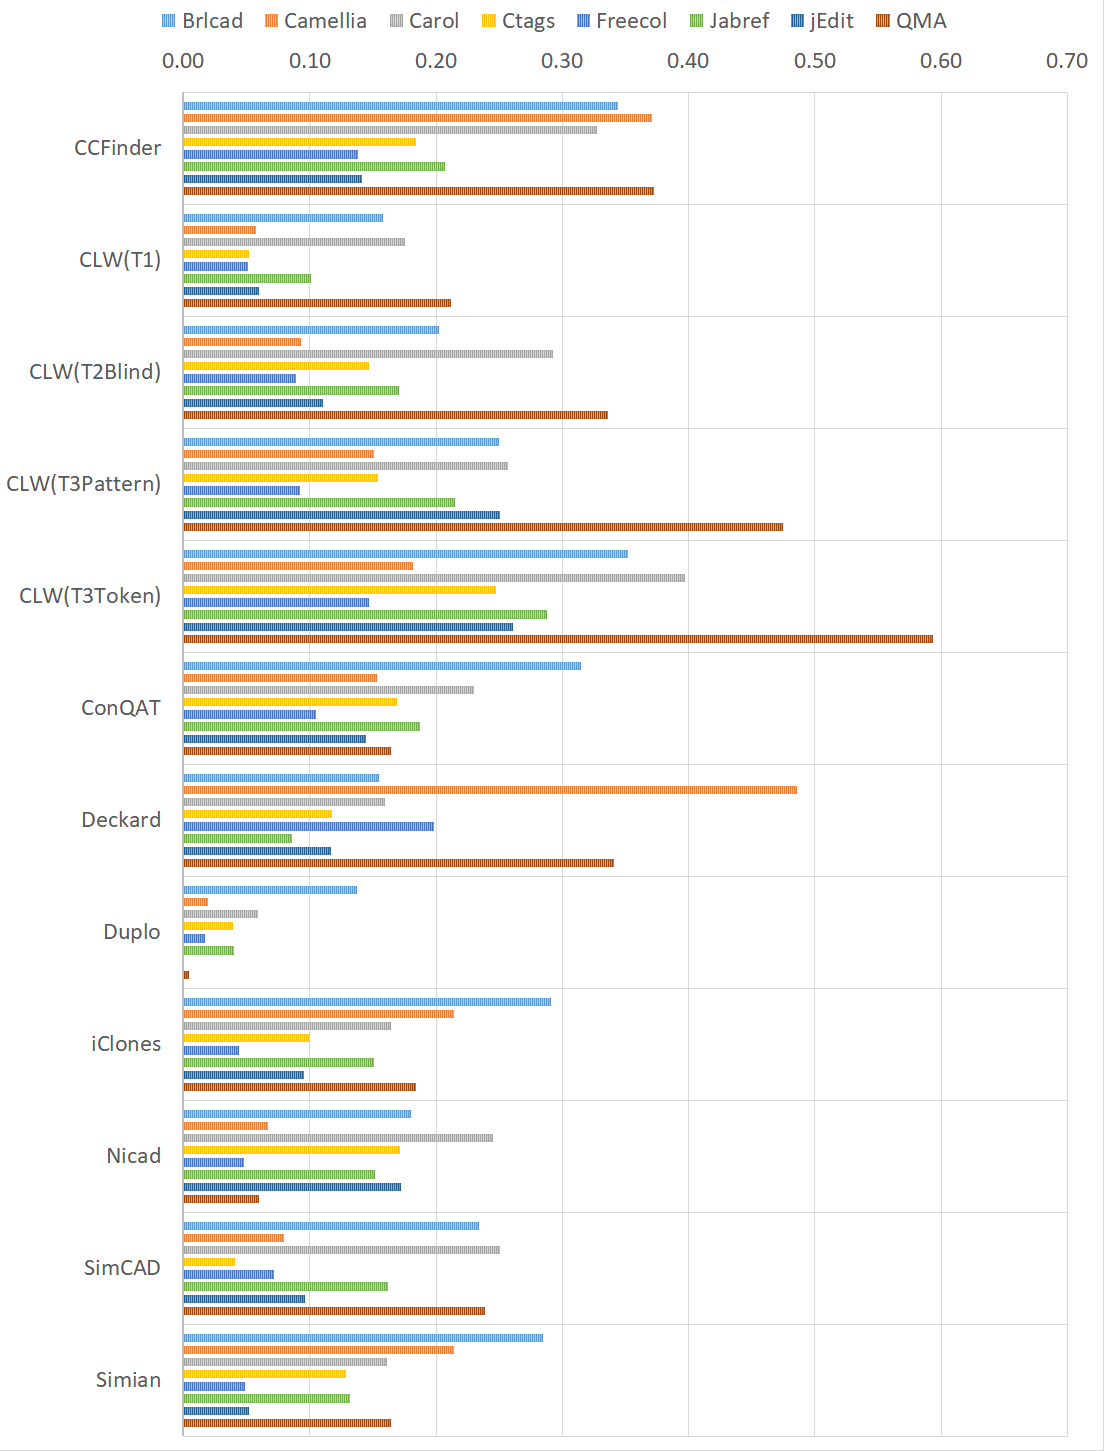
\includegraphics[width=\textwidth] {AveragePrecision.png}
% \caption{Average precision of different tools}
% \label{fig:AveragePrecision}
% \end{figure}
% %%% =================

%%%--- Bar Chart of AverageLineCoveredPerSS
\vspace{2mm}
\begin{figure}
\centering
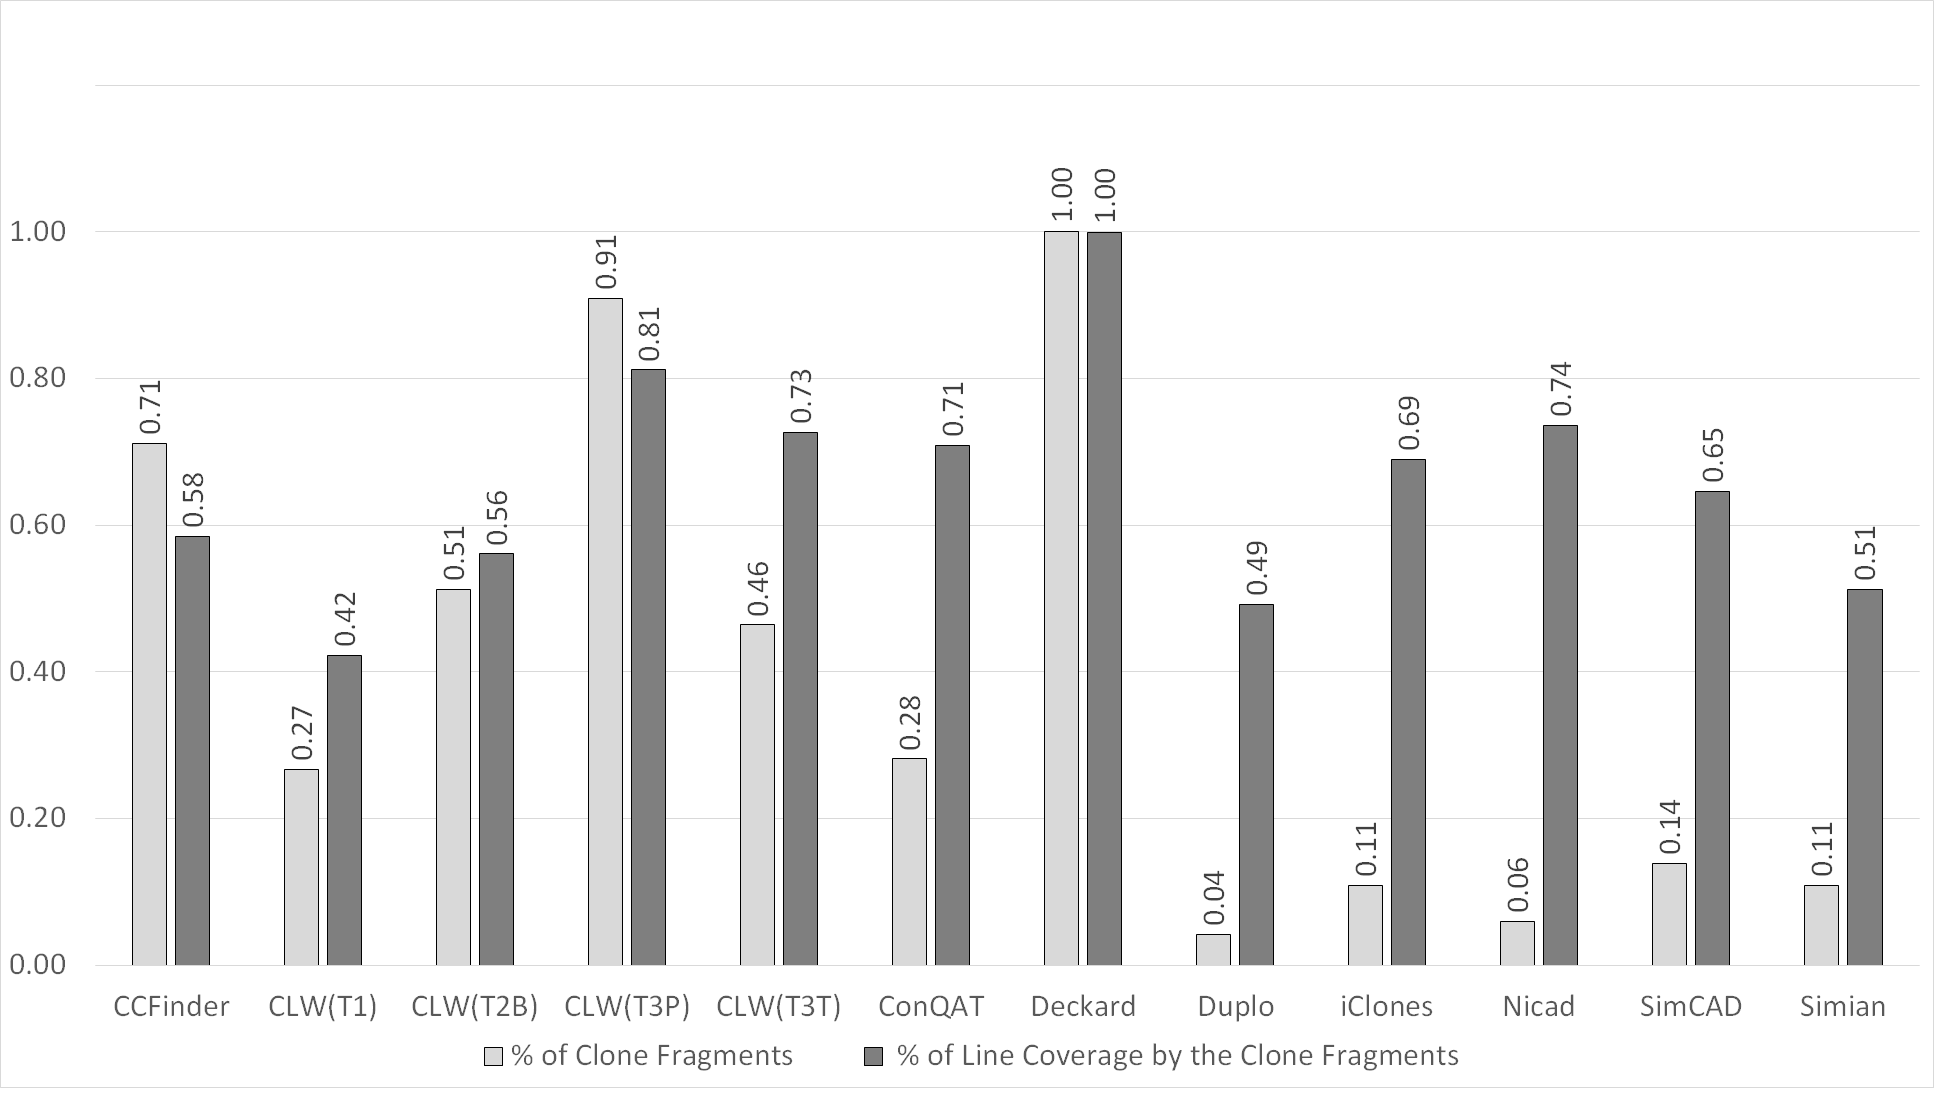
\includegraphics[width=\textwidth] {AverageLineCoveredPerSS.png}
% Calculation of Change Intersection: SELECT COUNT(`change_id`) FROM `pre_recall_conqat` WHERE `change_detect`>0
\caption{Comparing unique line coverage by clone fragments and number of clone fragments from different clone detectors.}
\label{fig:AverageLineCoveredPerSS}
\end{figure}
%%% =================
\subsection{Answer to the \textbf{RQ2}}
\textbf{What are the deciding factors for the performance variance of different clone detectors in detecting cloned co-change candidates?} 

From the answer of our \textbf{RQ1}, we found a difference in performance for different clone detection tools in suggesting cloned co-change candidates. We found a clone detection tool that performs well in detecting clone fragments may not be good at detecting cloned co-change candidates.  Such a scenario motivates us to find out the reason to answer this research question. 

We investigated the number of clone fragments and the number of unique lines covered by those clone fragments by all the 12 clone detectors from all the subject systems' revisions. Figure \ref{fig:AverageLineCoveredPerSS}  shows the comparison scenario of the number of clone fragments and lines covered by those clone fragments from different clone detectors. For better comparison, we bring the values on a single scale (between 0 and 1) where 0 and 1 represent the lowest and highest values, respectively, compared to all the clone detectors under comparison. Considering both, the number of clone fragments and the number of lines covered by those clone fragments from all the revisions of all the subject systems, if we order the clone detectors from the highest to the lowest, we find Deckard and CLW(T3P) in the top of the list. CLW(T3T) and CCFinder fall in the respective next position to provide the highest number of clone fragments and cover the highest number of unique lines in the source files. This scenario shows that a good clone detector can perform poorly in detecting cloned co-change candidates if it does not detect enough clone fragments and does not cover enough unique lines by those clone fragments in the source file. Though, earlier study \cite{Mondal-2014-PRC-2597073-2597104rankingCoChange} suggests that NiCad is an excellent clone detector in both of these cases, it falls at the bottom of the list. Even though NiCad performs very well in detecting clone fragments, it provides a lower number of clone fragments and also the lower number of line coverage by those clone fragments in the software systems. For that reason, while detecting the cloned co-change candidates, NiCad is showing lower F1~Score. The number of clone fragments and line coverage by those fragments seems to be an underlying factor behind the obtained comparison scenario of the clone detectors in predicting cloned co-change candidates. Some other factors such as (i) How clone fragments are overlapped with each other in a clone group? (ii) How is a clone detector determining the similarity among different fragments? (iii) What similarity score is used; it may also have an effect on the performance of predicting cloned co-change candidates. We plan to explore these factors in future studies.

\subsection{Answer to the \textbf{RQ3}}
\textbf{Do the source code processing techniques (Pattern/Token/Text-based processing) of the clone detection tools have any impact on their performance in detecting co-change candidates?}

We can answer this research question by analyzing our final ranking of the clone detectors in Table \ref{tab:final-ranking-sum-of-ranks}. Top two clone detectors of the final rank list (Rank 1 and 2) work by extracting source code patterns from the codebase. CLW(T3P) processes the source code terms by splitting into lines and then extracts code patterns. Deckard first generates vectors from the source file and then extracts a tree-like source pattern to match similarity among different source code fragments. The other five tools (Rank 3 to 7) in the rank list perform token-based source code processing, and the remaining five tools perform text-based source code processing for detecting clones from the source file. From this result, we can say that text-based clone detection tools are not suitable to be used in detecting cloned co-change candidates during software evolution. The tools which can detect more generalized clone fragments, especially pattern-based clone detectors, are perfect for detecting co-change candidates. 

\subsection{Answer to the \textbf{RQ4}}
\textbf{Do clone detection tools designed for detecting different types of clones (Type 1, 2, 3) work differently in detecting cloned co-change candidates?}

From the final rank list of our clone detectors, we also find the relation of detected clone types with its ability to detect cloned co-change candidates. The rank list of clone detectors in Table \ref{tab:final-ranking-sum-of-ranks} shows that clone detecting tools such as CLW(T1), Duplo, which detects the only Type 1 clone, will not perform well in detecting co-change candidates. On the other hand, tools such as CLW(T3P), CLW(T3T), Deckard, CCFinder perform very well in detecting cloned co-change candidates. The significance test results in Table \ref{tab:cochange-wilcoxon-rank-test} also show that four tools (two configurations of CloneWorks for Type-3, Deckard, and CCFinder) which perform significantly better than the other tools are also known as the clone detectors which detects Type-3 clones (Type-1 and Type-2 are also automatically included with Type-3 clones). Therefore, our findings suggest that we should choose those clone detectors to be used in detecting co-change candidates that detect Type-3 clones with the other Type-1 and Type-2 clone fragments. 

%%% Detection F1~Score of Cloned Co-change
\begin{table}[htbp]
\centering
%\small
\addtolength{\tabcolsep}{-4pt}
%\vspace{2mm}
\caption{\textsc{F1~Score of Different Tools in Detecting Cloned Co-change}}
\label{tab:detection-f1-score}
\begin{tabular}{|l|c|c|c|c|c|c|c|c|}
\hline
\multicolumn{1}{|c|}{\textbf{Tools/SS}} & \textbf{Brlcad} & \textbf{Camellia} & \textbf{Carol} & \textbf{Ctags} & \textbf{Freecol} & \textbf{Jabref} & \textbf{jEdit} & \textbf{QMA} \\ \hline \hline
CCFinder                                & 0.30            & 0.23              & 0.20           & 0.16           & 0.09             & 0.15            & 0.07           & 0.16         \\ \hline
CLW(T1)                                 & 0.09            & 0.04              & 0.06           & 0.03           & 0.03             & 0.05            & 0.04           & 0.11         \\ \hline
CLW(T2B)                            & 0.13            & 0.07              & 0.22           & 0.12           & 0.08             & 0.13            & 0.08           & 0.17         \\ \hline
CLW(T3P)                          & 0.32            & 0.16              & 0.36           & 0.25           & 0.15             & 0.30            & 0.35           & 0.49         \\ \hline
CLW(T3T)                            & 0.27            & 0.18              & 0.29           & 0.24           & 0.11             & 0.20            & 0.20           & 0.42         \\ \hline
ConQAT                                  & 0.28            & 0.10              & 0.12           & 0.15           & 0.08             & 0.12            & 0.08           & 0.08         \\ \hline
Deckard                                 & 0.19            & 0.57              & 0.21           & 0.15           & 0.30             & 0.14            & 0.18           & 0.41         \\ \hline
Duplo                                   & 0.12            & 0.01              & 0.03           & 0.03           & 0.01             & 0.02            & 0.00           & 0.00         \\ \hline
iClones                                 & 0.26            & 0.15              & 0.08           & 0.08           & 0.03             & 0.09            & 0.05           & 0.10         \\ \hline
Nicad                                   & 0.12            & 0.06              & 0.16           & 0.21           & 0.04             & 0.10            & 0.12           & 0.03         \\ \hline
SimCAD                                  & 0.17            & 0.07              & 0.15           & 0.04           & 0.05             & 0.10            & 0.06           & 0.10         \\ \hline
Simian                                  & 0.25            & 0.16              & 0.06           & 0.11           & 0.03             & 0.07            & 0.03           & 0.06         \\ \hline
\end{tabular}
\end{table}
%===============================

%%% Ranking Table
\begin{table}[htbp]
\caption{\textsc{Ranks of the clone detectors by considering individual ranking in each of the Subject Systems}}
\label{tab:final-ranking-sum-of-ranks}
\centering
%\addtolength{\tabcolsep}{-2pt}
\begin{tabular}{lcccccccccc}
\hline
\multicolumn{1}{|c|}{\textbf{\begin{tabular}[c]{@{}c@{}}Clone\\Detectors\end{tabular}}} & \multicolumn{1}{c|}{\textbf{S1}} & \multicolumn{1}{c|}{\textbf{S2}} & \multicolumn{1}{c|}{\textbf{S3}} & \multicolumn{1}{c|}{\textbf{S4}} & \multicolumn{1}{c|}{\textbf{S5}} & \multicolumn{1}{c|}{\textbf{S6}} & \multicolumn{1}{c|}{\textbf{S7}} & \multicolumn{1}{c|}{\textbf{S8}} & \multicolumn{1}{c|}{\textbf{\begin{tabular}[c]{@{}c@{}}$\sum_{S1}^{S8}$\end{tabular}}} & \multicolumn{1}{c|}{\textbf{\begin{tabular}[c]{@{}c@{}}Final\\ Rank\end{tabular}}} \\ \hline \hline
\multicolumn{1}{|l|}{\textbf{CLW(T3P)}}                                                   & \multicolumn{1}{c|}{1}           & \multicolumn{1}{c|}{4}           & \multicolumn{1}{c|}{1}           & \multicolumn{1}{c|}{1}           & \multicolumn{1}{c|}{2}           & \multicolumn{1}{c|}{1}           & \multicolumn{1}{c|}{1}           & \multicolumn{1}{c|}{1}           & \multicolumn{1}{c|}{12}                                                               & \multicolumn{1}{c|}{\textbf{1}}                                                    \\ \hline
\multicolumn{1}{|l|}{\textbf{CLW(T3T)}}                                                     & \multicolumn{1}{c|}{4}           & \multicolumn{1}{c|}{3}           & \multicolumn{1}{c|}{2}           & \multicolumn{1}{c|}{2}           & \multicolumn{1}{c|}{3}           & \multicolumn{1}{c|}{2}           & \multicolumn{1}{c|}{2}           & \multicolumn{1}{c|}{2}           & \multicolumn{1}{c|}{20}                                                               & \multicolumn{1}{c|}{\textbf{2}}                                                    \\ \hline
\multicolumn{1}{|l|}{\textbf{Deckard}}                                                          & \multicolumn{1}{c|}{7}           & \multicolumn{1}{c|}{1}           & \multicolumn{1}{c|}{4}           & \multicolumn{1}{c|}{6}           & \multicolumn{1}{c|}{1}           & \multicolumn{1}{c|}{4}           & \multicolumn{1}{c|}{3}           & \multicolumn{1}{c|}{3}           & \multicolumn{1}{c|}{29}                                                               & \multicolumn{1}{c|}{\textbf{3}}                                                    \\ \hline
\multicolumn{1}{|l|}{\textbf{CCFinder}}                                                         & \multicolumn{1}{c|}{2}           & \multicolumn{1}{c|}{2}           & \multicolumn{1}{c|}{5}           & \multicolumn{1}{c|}{4}           & \multicolumn{1}{c|}{4}           & \multicolumn{1}{c|}{3}           & \multicolumn{1}{c|}{7}           & \multicolumn{1}{c|}{5}           & \multicolumn{1}{c|}{32}                                                               & \multicolumn{1}{c|}{\textbf{4}}                                                    \\ \hline
\multicolumn{1}{|l|}{\textbf{CLW(T2B)}}                                                     & \multicolumn{1}{c|}{9}           & \multicolumn{1}{c|}{8}           & \multicolumn{1}{c|}{3}           & \multicolumn{1}{c|}{7}           & \multicolumn{1}{c|}{5}           & \multicolumn{1}{c|}{5}           & \multicolumn{1}{c|}{5}           & \multicolumn{1}{c|}{4}           & \multicolumn{1}{c|}{46}                                                               & \multicolumn{1}{c|}{\textbf{5}}                                                    \\ \hline
\multicolumn{1}{|l|}{\textbf{ConQAT}}                                                           & \multicolumn{1}{c|}{3}           & \multicolumn{1}{c|}{7}           & \multicolumn{1}{c|}{8}           & \multicolumn{1}{c|}{5}           & \multicolumn{1}{c|}{6}           & \multicolumn{1}{c|}{6}           & \multicolumn{1}{c|}{6}           & \multicolumn{1}{c|}{9}           & \multicolumn{1}{c|}{50}                                                               & \multicolumn{1}{c|}{\textbf{6}}                                                    \\ \hline
\multicolumn{1}{|l|}{\textbf{iClones}}                                                          & \multicolumn{1}{c|}{11}          & \multicolumn{1}{c|}{10}          & \multicolumn{1}{c|}{6}           & \multicolumn{1}{c|}{3}           & \multicolumn{1}{c|}{8}           & \multicolumn{1}{c|}{7}           & \multicolumn{1}{c|}{4}           & \multicolumn{1}{c|}{11}          & \multicolumn{1}{c|}{60}                                                               & \multicolumn{1}{c|}{\textbf{7}}                                                    \\ \hline
\multicolumn{1}{|l|}{\textbf{Simian}}                                                           & \multicolumn{1}{c|}{5}           & \multicolumn{1}{c|}{6}           & \multicolumn{1}{c|}{9}           & \multicolumn{1}{c|}{9}           & \multicolumn{1}{c|}{10}          & \multicolumn{1}{c|}{9}           & \multicolumn{1}{c|}{9}           & \multicolumn{1}{c|}{7}           & \multicolumn{1}{c|}{64}                                                               & \multicolumn{1}{c|}{\textbf{8}}                                                    \\ \hline
\multicolumn{1}{|l|}{\textbf{Nicad}}                                                            & \multicolumn{1}{c|}{8}           & \multicolumn{1}{c|}{9}           & \multicolumn{1}{c|}{7}           & \multicolumn{1}{c|}{10}          & \multicolumn{1}{c|}{7}           & \multicolumn{1}{c|}{8}           & \multicolumn{1}{c|}{8}           & \multicolumn{1}{c|}{8}           & \multicolumn{1}{c|}{65}                                                               & \multicolumn{1}{c|}{\textbf{9}}                                                    \\ \hline
\multicolumn{1}{|l|}{\textbf{SimCAD}}                                                           & \multicolumn{1}{c|}{6}           & \multicolumn{1}{c|}{5}           & \multicolumn{1}{c|}{11}          & \multicolumn{1}{c|}{8}           & \multicolumn{1}{c|}{11}          & \multicolumn{1}{c|}{10}          & \multicolumn{1}{c|}{11}          & \multicolumn{1}{c|}{10}          & \multicolumn{1}{c|}{72}                                                               & \multicolumn{1}{c|}{\textbf{10}}                                                   \\ \hline
\multicolumn{1}{|l|}{\textbf{CLW(T1)}}                                                          & \multicolumn{1}{c|}{12}          & \multicolumn{1}{c|}{11}          & \multicolumn{1}{c|}{10}          & \multicolumn{1}{c|}{11}          & \multicolumn{1}{c|}{9}           & \multicolumn{1}{c|}{11}          & \multicolumn{1}{c|}{10}          & \multicolumn{1}{c|}{6}           & \multicolumn{1}{c|}{80}                                                               & \multicolumn{1}{c|}{\textbf{11}}                                                   \\ \hline
\multicolumn{1}{|l|}{\textbf{Duplo}}                                                            & \multicolumn{1}{c|}{10}          & \multicolumn{1}{c|}{12}          & \multicolumn{1}{c|}{12}          & \multicolumn{1}{c|}{12}          & \multicolumn{1}{c|}{12}          & \multicolumn{1}{c|}{12}          & \multicolumn{1}{c|}{12}          & \multicolumn{1}{c|}{12}          & \multicolumn{1}{c|}{94}                                                               & \multicolumn{1}{c|}{\textbf{12}}                                                   \\ \hline
\multicolumn{11}{l}{\textit{\begin{tabular}[c]{@{}l@{}}\textbf{* S1-S8} represents sequence of eight subject systems used in this study.\end{tabular}}}                                                                                                                                                                                                                                                                                                                                                                                                          
\end{tabular}
\end{table}
%%% ==================================================

%%%--- CochangeBoxFScoresRanked
\begin{figure}
\centering
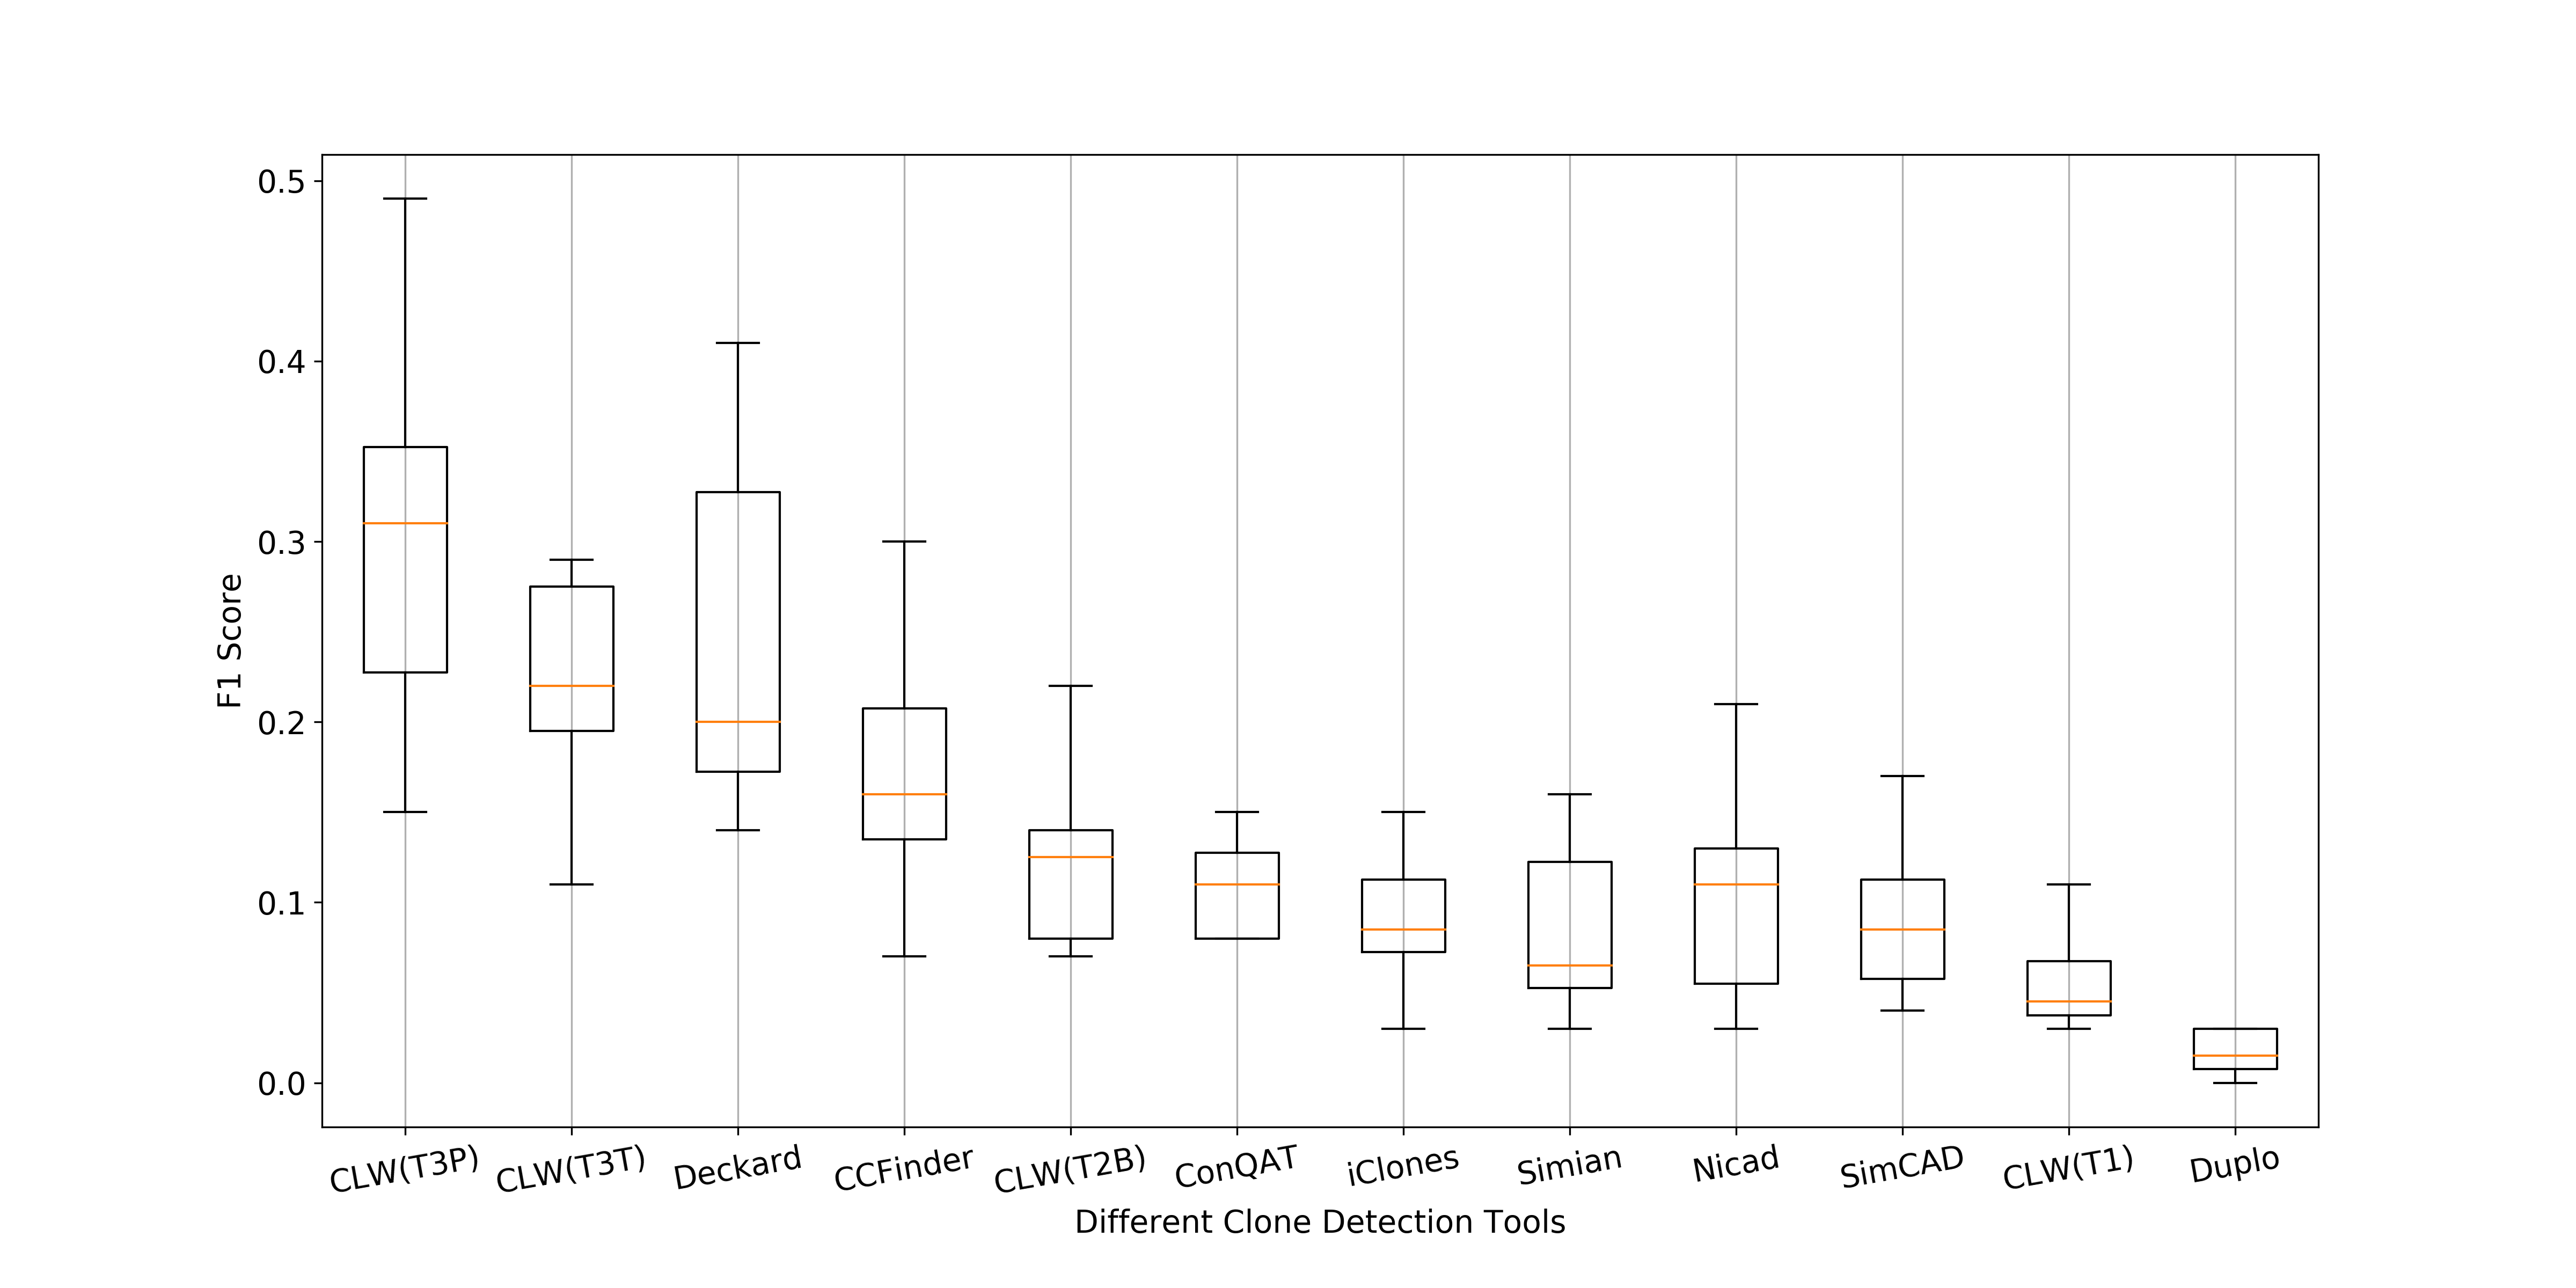
\includegraphics[width=\textwidth] {CochangeBoxFScoresRanked.png}
\caption{Comparing Distribution of F1~Scores in Different Clone Detectors}
\label{fig:CochangeBoxFScoresRanked}
\end{figure}
%%% =================

%%%%%%%%%%% Significance (Wilcoxon Signed Rank Test) Test %%%%%%%%%%%%%%%%%%%%%%%%
\begin{table}[htbp]
\caption{\textsc{Wilcoxon Signed Rank Test (p<0.05)}}
\label{tab:cochange-wilcoxon-rank-test}
\centering
%\addtolength{\tabcolsep}{0pt}
\begin{tabular}{|l|l|l|l|l|l|l|l|l|l|l|c|}
\hline
\multicolumn{1}{|c|}{\textbf{\begin{tabular}[c]{@{}c@{}}Tools in \\ Investigation\end{tabular}}} & \multicolumn{10}{c|}{\textbf{\begin{tabular}[c]{@{}c@{}}Significantly Better than \\ Tools (p\textless{}0.05)\end{tabular}}}                                    & \textbf{\begin{tabular}[c]{@{}c@{}}\# of \\ Tools\end{tabular}} \\ \hline \hline
\textbf{CLW(T3P)}                                                                          & \multicolumn{10}{l|}{\begin{tabular}[c]{@{}l@{}}CLW(T3T), CCFinder, CLW(T2B), \\ ConQAT, iClones, Simian, Nicad, SimCAD,\\ CLW(T1), Duplo\end{tabular}} & 10                                                              \\ \hline
\textbf{CLW(T3T)}                                                                            & \multicolumn{10}{l|}{\begin{tabular}[c]{@{}l@{}}CLW(T2B), ConQAT, iClones, Simian,\\ Nicad, SimCAD, CLW(T1), Duplo\end{tabular}}                            & 8                                                               \\ \hline
\textbf{Deckard}                                                                                 & \multicolumn{10}{l|}{\begin{tabular}[c]{@{}l@{}}CLW(T2B), iClones, Simian, Nicad, \\ SimCAD, CLW(T1), Duplo\end{tabular}}                                   & 7                                                               \\ \hline
\textbf{CCFinder}                                                                                & \multicolumn{10}{l|}{\begin{tabular}[c]{@{}l@{}}ConQAT, iClones, Simian, \\ SimCAD, CLW(T1), Duplo\end{tabular}}                                                & 6                                                               \\ \hline
\textbf{CLW(T2B)}                                                                            & \multicolumn{10}{l|}{CLW(T1), Duplo}                                                                                                                            & 2                                                               \\ \hline
\textbf{ConQAT}                                                                                  & \multicolumn{10}{l|}{CLW(T1), Duplo}                                                                                                                            & 2                                                               \\ \hline
\textbf{iClones}                                                                                 & \multicolumn{10}{l|}{CLW(T1), Duplo}                                                                                                                            & 2                                                               \\ \hline
\textbf{Simian}                                                                                  & \multicolumn{10}{l|}{Duplo}                                                                                                                                     & 1                                                               \\ \hline
\textbf{Nicad}                                                                                   & \multicolumn{10}{l|}{Duplo}                                                                                                                                     & 1                                                               \\ \hline
\textbf{SimCAD}                                                                                  & \multicolumn{10}{l|}{CLW(T1), Duplo}                                                                                                                            & 2                                                               \\ \hline
\end{tabular}
\end{table}
%================================================================================

\subsection{The Wilcoxon Signed-Rank Test:}
\label{sec-wilcoxon-singed-rank-test}
We performed The Wilcoxon Signed-Rank Test \cite{wilcoxon-signed-rank-test, wilcoxon-signed-rank-test-rosner} to verify the hypothesis that the F1~Scores of a tool which has obtained a higher rank in Table \ref{tab:final-ranking-sum-of-ranks} are significantly different (better) than the F1~Scores of the tools which have got lower ranks. Here, F1~Scores of each tool contains eight values obtained in all the eight subject systems. For instance, let us assume that we would like to examine whether the F1~Scores obtained by CLW(T3P) are significantly better than the F1~Scores obtained by CLW(T3T). Thus, we take the sets of F1~Scores (see Table \ref{tab:detection-f1-score}) from both CLW(T3P) and CLW(T3T), which will be then used to perform Wilcoxon Signed-Rank Test utilizing the SciPy library \cite{SciPy-NMeth2020} available in Python programming language. We did a significance test for each of the possible pairs from all the 12 clone detection tools in our investigation. 

A summary of the significant results at $p<0.05$ obtained from the significance test is given in Table \ref{tab:cochange-wilcoxon-rank-test}. The left-most column of this table contains the tool whose significance is to be tested, and the next column contains the name of the tools, each of them provides significantly different F1~Scores compared to the tool in the investigation. The right-most column of Table \ref{tab:cochange-wilcoxon-rank-test} shows the number of clone detectors whose F1~Scores are significantly different from the F1~Scores of the tool under investigation. Therefore, CLW(T3P) provides significantly different F1~Scores than 10 other clone detectors (excluding Deckard). The distribution of F1~Scores in Figure \ref{fig:CochangeBoxFScoresRanked} also shows that majority of the F1~Score values of CLW(T3P) lie above all the other clone detectors'  F1~Score values (except Deckard). Although some of the F1~Socre values in CLW(T3P) are above Deckard's values, those are not enough to make the result significantly different. This scenario clearly shows that CLW(T3P) is significantly better than all the other clone detectors except Deckard. Similarly, from the following results of our significance test in Table \ref{tab:cochange-wilcoxon-rank-test}, we can see that F1~Scores of CLW(T3T) are significantly better than the other eight clone detectors, F1~Scores of Deckard are significantly better than the other seven clone detectors, and F1~Scores of CCFinder are significantly better than the other six clone detectors. The following four tools (CLW(T2B), ConQAT, iClones, SimCAD) are significantly better than CLW(T1) and Duplo. Simian and NiCad are significantly better than only Duplo. The overall observation of the significance test result helps to conclude that for detecting clone co-change candidates, CloneWorks Type-3 clone detection configuration can be an excellent choice, Deckard and CCFinder are also good choices. However, the other tools are not significantly better choices to detect co-change candidates during software evolution. 

The distribution of F1~Scores in Figure \ref{fig:CochangeBoxFScoresRanked} also demonstrates the significance in performance differences of clone detectors used in this study. The clone detectors in this figure are sorted based on the final rank list shown in Table \ref{tab:final-ranking-sum-of-ranks}, where the ranks of the tools are presented from left to right (rank 1 to 12 in Table \ref{tab:final-ranking-sum-of-ranks}). This figure shows the clone detectors which got higher ranking in Table \ref{tab:final-ranking-sum-of-ranks} also have the higher values of F1~Scores compared to the tools which are below in the rank list. In this diagram, we can see that the F1~Scores of CloneWorks Type-3 Pattern have the most higher values, and Duplo has the most lower values in their respective distributions. Any two tools' performance will be significantly different from each other if they share a fewer common range of F1~Scores distribution. From the result of the significance test in Table \ref{tab:cochange-wilcoxon-rank-test}, we can see that Deckard is not significantly different from all the other three good clone detectors i.e. CLW(T3P), CLW(T3T), and CCFinder as they share most of the same range of values in the distribution. We can see a similar scenario for Simian and Nicad, e.g., though Simian and Nicad are above four and three other clone detectors, their F1~Scores are significantly better than only Duplo. Simian, Nicad, SimCad, CLW(T1) shares most of the same range of values in the distribution of F1~Scores. Therefore, they do not provide a significantly different result with each other. 

\section{Discussion}
\label{the-discussion}
There are two primary perspectives of managing code clones: (1) clone tracking and (2) clone refactoring. Our research principally focuses on the clone tracking perspective. A clone tracker's main task is to suggest similar co-change candidates when a programmer attempts to change a code fragment. For suggesting co-change candidates, a clone tracker depends on a clone detector. Our research compares 12 promising clone detectors based on their capabilities in suggesting cloned co-change candidates. According to our investigation, CloneWorks (Type-3 Pattern, and Type-3 Token), Deckard, and CCFinder are the most promising tools for suggesting such co-change candidates based on the ranking we obtained in Table \ref{tab:final-ranking-sum-of-ranks} and the result of our significance test in Table \ref{tab:cochange-wilcoxon-rank-test}. Based on our overall observation, we can say that the performance of CloneWorks (Type-3 Pattern/ Token), Deckard, and CCFinder are much better compared to the other clone detection tools in detecting co-change candidates during software evolution. As the clone classes/ pairs generated by different clone detectors played an essential role in our analysis, we can say that the clone detectors which can group similar clone fragments into a clone class/ pair efficiently will perform better in detecting co-change candidates during the commit operation. From our findings, we can also say that the clone detectors which detect all the clone types such as Type-1, Type-2, and Type-3 clones can also perform well in detecting co-change candidates. 

When a particular code fragment is changed, we apply the clone detectors to predict which other similar code fragments might need to be co-changed. However, some different fragments might also be changed together with the particular fragment. As we apply only clone detectors, we cannot consider those dissimilar co-change candidates in our research. We only apply our analysis to those change candidates whose co-changes are detected by at least one (out of 12) clone detection techniques in our investigation. We believe, removing the change candidates whose co-change is not detected by any of the clone detectors lead to removing the independent changes (which should not be subject in the co-change related study) from our analysis.  This removal also leads to making a fair comparison among the clone detectors in this study.

In our research, we do not compare the clone detectors considering their clone detection efficiency. We instead compare the clone detection tools based on their ability to suggest cloned co-change candidates. Such a comparison of clone detectors focusing on a particular maintenance perspective was not made previously. Suggesting co-change candidates for a target program entity is a vital impact analysis \cite{book-change-impact} task during software evolution. Thus, through our research, we investigate which of the clone detectors can be useful in change impact analysis to what extent. Findings from our research can not only identify which clone detector(s) can be promising for change impact analysis by finding the cloned co-change candidates but also it can contribute in finding possible fixes of inconsistencies in software systems by analyzing historical inconsistencies (due to missing the change in cloned co-change candidates) and their fixes.  

\section{Threats to Validity}
\label{the-threat-validity}
This study's findings are based on the investigation of 12 clone detection techniques on eight subject systems. The inclusion of more subject systems may increase the generalizability of the findings. The decision to select subject systems are based on the variety, popularity, used programming languages, and availability of a considerable number of revisions. The subject systems used in this study are of the two most popular programming languages and of different application domains, sizes, and revision history lengths, which makes the obtained results generalizable. We believe our results are not biased by our choice of subject systems and are distinguished from software maintenance perspectives.

The parameters to detect clone fragments used in the 12 clone detectors may impact the comparison scenario in this study. However, we considered taking equivalent configurations to minimize such impact. Therefore, we believe comparing different clone detectors based on their detected cloned fragments and the cloned co-change candidate is made without any influence of their clone detection configurations. 

Several code fragments might change together in a commit operation. While some of these fragments can be similar to one another, and some might be dissimilar. Similar code fragments co-change (i.e., change together) for ensuring consistency of the codebase. However, dissimilar code fragments can co-change because of their underlying dependencies, which could impact the generalization of this research outcome. As we aim to compare the clone detection tools, we wanted to discard the dissimilar co-change candidates from our consideration. If a co-change candidate was not detected as a true positive by any of the clone detectors, we discarded the candidate. We believe that such a consideration is reasonable in our experiment aiming towards comparing clone detectors, and our findings may inspire more similar research.

\section{Conclusion and Future Works}
\label{the-conclusion-cochange}
In this research, we compare different clone detection tools from the perspective of software maintenance. In particular, we investigate their performances in successfully suggesting (i.e., predicting) cloned co-change candidates during evolution. We used eight open-source subject systems written in C and Java for our analysis. According to our final rank list in Table \ref{tab:final-ranking-sum-of-ranks} and summary of significance test result in Table \ref{tab:cochange-wilcoxon-rank-test}, show that both the configurations (Pattern and Token) of CloneWorks clone detection tool for detecting type-3 clones are performing significantly better compared to more than 72\% other clone detectors used in this study. Deckard and CCFinder are also better compared to more than 55\% of the other tools. CloneWorks (Type-2), ConQAT, iClones are also showing better performance than the other remaining tools. Although we have figured some reasons of the better performance of Deckard, CloneWorks, and CCFinder in this extensive study, we plan to do some future related works by analyzing the internal mechanism of clone detection tools to find out how the change of these mechanisms are effecting the detection of cloned co-change candidates. We also want to investigate the impact of different similarity scores of different clone detectors in finding co-change candidates in our future work. Besides, we want to include some other software systems of different programming languages (i.e., C\#, Python) in our future research.

\section*{Acknowledgment}
This research is supported by the Natural Sciences and Engineering Research Council of Canada (NSERC), and by a Canada First Research Excellence Fund (CFREF) grant coordinated by the Global Institute for Food Security (GIFS).



%\section*{References}
\bibliography{mybibfile}

\end{document}